\documentclass[12pt,oneside]{memoir} 

% Paket koji definiše sve specifičnosti master rada Matematičkog fakulteta
\usepackage[latinica,biblatex]{matfmaster} 
\usepackage{csquotes}
\usepackage{listings}
\usepackage[compatibility=false]{caption}
\usepackage{subcaption}
\usepackage[cache=false]{minted}
\usemintedstyle{friendly}
\AtEndEnvironment{listing}{\vspace{-15pt}}
\usepackage{xcolor}

% Podrazumevano pismo je ćirilica.

% Datoteka sa literaturom u BibTex tj. BibLaTeX/Biber formatu
\bib{teza} 

% Ime kandidata na srpskom jeziku (u odabranom pismu)
\autor{Nemanja Subotić} 
% Naslov teze na srpskom jeziku (u odabranom pismu)
\naslov{Programski jezici Elm i Elixir u razvoju studentskog veb portala}
% Godina u kojoj je teza predana komisiji
\godina{2020}
% Ime i afilijacija mentora (u odabranom pismu)
\mentor{dr Milena \textsc{Vujošević Janičić}, docent    \\ Univerzitet u Beogradu, Matematički fakultet}
% Ime i afilijacija prvog člana komisije (u odabranom pismu)
\komisijaA{dr Filip \textsc{Marić}, vanredni profesor\\ Univerzitet u Beogradu, Matematički fakultet}
% Ime i afilijacija drugog člana komisije (u odabranom pismu)
\komisijaB{dr Ivan \textsc{Čukić}, docent\\ Univerzitet u Beogradu, Matematički fakultet}
% Ime i afilijacija trećeg člana komisije (opciono)
% \komisijaC{}
% Ime i afilijacija četvrtog člana komisije (opciono)
% \komisijaD{}
% Datum odbrane (odkomentarisati narednu liniju i upisati datum odbrane ako je poznat)
% \datumodbrane{}

% Apstrakt na srpskom jeziku (u odabranom pismu)
\apstr{%
Apstrakt rada
}

% Ključne reči na srpskom jeziku (u odabranom pismu)
\kljucnereci{elm, elixir, ...}

\begin{document}
% ==============================================================================
% Uvodni deo teze
\frontmatter
% ==============================================================================
% Naslovna strana
\naslovna
% Strana sa podacima o mentoru i članovima komisije
\komisija
% Strana sa podacima o disertaciji na srpskom jeziku
\apstrakt
% Sadržaj teze
\tableofcontents*

% ==============================================================================
% Glavni deo teze
\mainmatter
% ==============================================================================

% ------------------------------------------------------------------------------
\chapter{Uvod}
% ------------------------------------------------------------------------------

Funkcionalno programiranje kao programska paradigma nastaje 1959.godine sa
pojavom LISP-a, prvog funkcionalnog programskog jezika...
 Elm... Phoenix i Elixir... MSNR Poral...

\chapter{Programski jezik i okruženje Elm}
Evan Zaplicki (Evan Czaplicki) je 2012. godine objavio svoju tezu "Elm: Konkurento FRP
\footnote{FRP je skraćenica za funkcionalno reaktivno programiranje} za funkcionalne GUI-je
\footnote{GUI je skraćenica za grafički korisnički interfjes}" (eng. \emph{"Elm: Concurrent
FRP for Functional GUIs"}) \cite{elm:2012} i, s ciljem da GUI programiranje učini
prijatnijim, dizajnirao novi programski jezik --- Elm. Na slici \ref{fig:elm-logo} prikazan
je logo jezika.
Elm je statički tipiziran, čisto funkcionalni programski jezik koji se
kompilira, tačnije transpilira u JavaScript i namenjen je isključivo za
kreiranje korisničkog interfjesa veb aplikacija.
\begin{figure}[!ht]
  \centering
  
\includegraphics[width=0.3\textwidth]{elm.png}
  \caption{Logo programskog jezika Elm}
  \label{fig:elm-logo}
\end{figure}
Takođe, Elm nije samo programski jezik već i platforma za razvoj aplikacija.
Zbog svoje funkcionalne prirode i prisustva kompilatora, Elm spada među
najstabilnija i najpouzdanija razvojna okruženja, a za Elm aplikacije važi
da, u praksi, ne izbacuju neplanirane greške tokom izvršavanja (eng. \emph{No 
Runtime Exceptions}).

\section{Uputstvo za instlaciju}
Pored želje da frontend programiranje učini prijatnijim, kreator jezika nastoji 
da ono bude i pristupačnije. Stoga, da bi se počelo sa korišćenjem Elma instalacija 
nije potrebna, dovoljeno je otići na zvaničnu veb stranicu i pokrenuti dostupan 
interaktivni kompilator \cite{tryelm}, gde se može naći dosta primera, kao i vodič kroz Elm.

Za zahtevnije projekte neophodno je izvršiti instalaciju, koja je vrlo
jednostavna. Potrebno je pratiti instrukcije sa zvanične stranice
\cite{installelm}. Takođe, moguća je instalacija pomoću \textbf{npm}
\footnote{npm --- \emph{Node Package Manager} predstavlja alat za upravljanje paketima u 
JavaScript programskom jeziku} alata \cite{npm}.
Na slici \ref{fig:elm-cmd} prikazana je provera uspešne instalacije, koja se može izvršiti
pokretanjem komande \textbf{elm} u komandnoj liniji, gde će se prikazati poruka
dobrodošlice i spisak mogućih komandi o kojima će biti reč u sledećim poglavljima.
\begin{figure}[!ht]
  \centering
  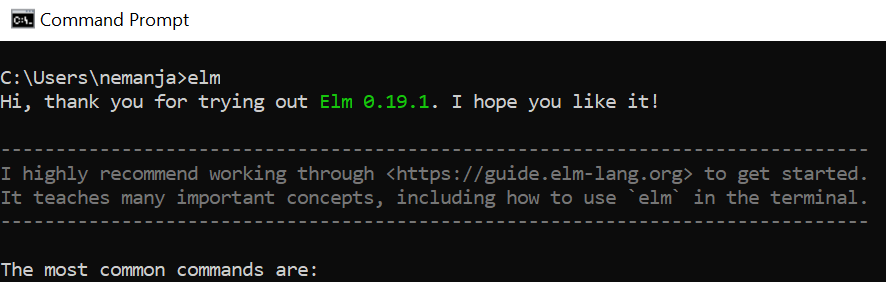
\includegraphics[width=0.95\textwidth]{elm-cmd.png}
  \caption{Provera uspešne instalacije Elma}
  \label{fig:elm-cmd}
\end{figure}

\section{Osnovne odlike}
Pored \emph{No Runtime Exceptions}, jedna od glavnih odlika ovog jezika jeste
kompilator, koji je izuzetno ugodan za rad. Mnogi programeri smatraju da Elm
kompilator proizvodi najbolje poruke o greškama. Za razliku od drugih, Elm
kompilator objašnjava zašto je došlo do greške i daje predloge za njihovo rešavanje,
a takođe nema kaskadnih poruka. Kreator se vodio razmišljanjem da kompilator treba
da bude asistent, ne samo alat.

Elm koristi svoju verziju \emph{virtuelnog DOM\footnote{DOM --- Obejektni model
dokumenta (eng. \emph{Document Object Model})\cite{dom}}-a}, koncepta koji se koristi u mnogim
frontend okruženima. Ideja je da se u memoriji čuva "virtuelna" reprezentacija
korisničkog interfejsa na osnovu koje se ažurira "stvarni" DOM. Još jedna bitna
karakteristika Elma je nepromenljivost podataka, što znači da se jednom definisani
podaci ne mogu više menjati. Direktna posledica nepromenljivosti podataka je veoma
brzo renderovanje HTML-a, jer se poređenja u virtuelnom DOM-u mogu vršiti po referenci. 
Verzija Elm 0.17 imala je najbrže renderovanje u poređenju sa tadašnjim aktuelnim verzijama 
popularnih okruženja\cite{elm-html}.

Elm se može integrisati i u postojeće JavaScript projekte za implementaciju pojedinačnih 
komponenti. Takođe, moguća je i komunikacija između Elma i JavaScripta. 

\section{Elm kao platforma}
Elm sa sobom donosi niz alata (tabela \ref{table:1}) i Elm okruženje (eng. \emph{Elm 
Runtime}), koji su neophodni za razvoj i izvršavanje aplikacija. Elm k\^{o}d se nalazi u 
datotekama sa \emph{.elm} ekstenzijom i prilikom kompilacije kreira se jedna izlazna 
\emph{.js} datoteka. U izlaznoj datoteci se pored prevedenog koda iz ulaznih \emph{.elm} 
datoteka nalaze i funkcije iz Elm okruženja potrebne za izvršavanje programa.

\begin{table}[h!]
\centering
\begin{tabular}{|l l|} 
 \hline 
 Alati & Kratat opis  \\ [0.5ex] 
 \hline
  \textbf{repl} & Pokretanje interaktivne sesije (eng. \emph{Read-Eval-Print-Loop}) \\ 
  \textbf{init} & Inicijalizacija projekta \\
  \textbf{reactor} & Pokretanje lokalnog servera \\
  \textbf{make} & Upotreba kompilatora \\
  \textbf{install}  & Preuzimanje paketa \\ 
  \textbf{diff} & Prikazivanje razlika između različitih verzija istog paketa \\
  \textbf{bump} & Određivanje broja naredne verzije paketa  \\
  \textbf{publish} & Objavljivanje paketa \\[1ex] 
 \hline
\end{tabular}
\caption{Elm alati komandne linije}
\label{table:1}
\end{table}

 
Kao zaseban jezik Elm ima i zaseban sistem za upravljanje paketima.
Pokretanjem komande \textbf{elm init} kreira se prazan \emph{src} direktorijum i 
datoteka \emph{elm.json}, u kojoj se pored informacije o tipu projekta (aplikacija ili 
paket), Elm verzije i liste direktorijuma sa kodom, nalazi i spisak paketa koji se 
koriste u projektu. Dodavanje novog paketa se vrši pomoću komande \textbf{elm install} 
\emph{naziv-paketa}. Svi paketi su javno dostupni (\url{https://package.elm-lang.org/}),
nazivi paketa su oblika \emph{autor/ime-paketa}.

Kompilacija se vrši naredbom \textbf{elm make} \emph{<jedna-ili-više-elm-datoteka>},
ukoliko se ne navede izlazna datoteka pomoću argumenta \emph{-{}-output} generisaće 
se \emph{index.html} datoteka sa prevedenim JavaScript kodom. Ostali argumenti kao i
više informacija o drugim alatima mogu se videti pomoću naredbe \textbf{elm} 
\emph{naziv-alata} \textbf{-{}-help}

\section{Elm kao jezik}
Kao i većina statički tipiziranih funkcionalnih programskih jezika, Elm se zasniva na
programskom jeziku ML, a budući da su u programskom jeziku Haskell napisani Elm kompilator
i ostali alati, Haskell je ostavio veliki uticaj i na sam jezik. Autor Elma smatra:
\begin{displayquote}
"Rekao bih da je Elm ML sa sintaksom poput Haskell-a. Ako poredimo semantiku, Elm je
dosta sličniji OCaml-u i SML-u." \cite{eczaplicki:2015}
\end{displayquote}

\textbf{ML} (eng. \emph{Meta Language})\cite{ml} je statički tipiziran programski jezik opšte 
namene koji je nastao 1973. godine na Univerzitetu u Edinburgu. Vođa grupe koja je radila
na dizajniranju programskog jezika ML bio je Robin Milner, dobitnik Tjuringove nagrade.
Nastao je pod uticajem programskog jezika LISP, a razvijan je za implementiranje automatskog
dokazivača teorema. Osnovna karakteristika jeste uvođenje automatskog zaključivanja tipova, a
odlikuje ga i poklapanje obrazaca, Karijeve funkcije i posedovanje sakupljača otpadaka. ML
nije čist funkcionalan  jezik i nema ugrađenu podršku za lenjo izračunavanje. U porodicu ML 
jezika, između ostalih, spadaju i \textbf{Standard ML}, \textbf{OCaml} i \textbf{F{\#}}.


\textbf{Haskell}\cite{haskell} je čist funkcionalni programski, naziv je dobio po matematičaru i 
logičaru Haskelu Bruks Kariju (eng. \emph{Haskell Brooks Curry}). Haskell je strogo 
tipiziran, poseduje automatsko zaključivanje tipova i lenjo izračunavanje. Jezik je 
opšte namene, pruža podršku za paralelno i distirbuirano programiranje. Haskell 
omogućava manje grešaka i veću pouzdanost kroz kraći i čistiji k\^{o}d, koji je lakši za
održavanje. 


\subsection{Komentari}
Komentari se u Elmu mogu navoditi na dva načina: \begin{itemize}
  \item Korišćenjem \texttt{-{}-} za linijske komentare
  \item Navođenjem teksta između znakova \texttt{\{-} i \texttt{-\}} za komentare u više redova.    
\end{itemize}

\subsection{Osnovni tipovi podataka}
\begin{listing}[h]
\begin{minted}{haskell}
> 'Z'
'Z' : Char
> "Zdravo!"
"Zdravo!" : String
> True
True : Bool
>42
42 : number
> 42 / 10 
4.2 : Float
> 42 // 10 --celobrojno deljenje
4 : Int
\end{minted}
\caption{Osnovni tipovi podataka prikazani u interpreteru}
\label{listing:tipovi}
\end{listing}
Osnovni tipovi podataka u Elmu su \textbf{Char}, \textbf{String}, \textbf{Bool},
\textbf{Int} i \textbf{Float}. U listingu \ref{listing:tipovi} prikazani su osnovni
tipovi korišćenjem interpretera (\texttt{\textbf{elm repl}}). Budući da i Elm poseduje zaključivanje tipova, nakon
izračunate vrednosti unetog izraza ispisuje se tip. U konkretnom primeru broj 42 se
može posmartati i kao tip \textbf{Int} i kao tip \textbf{Float}, pa interpreter vraća
\texttt{number} kao tip, iako \texttt{number} nije konkretan tip podataka.


Tip \textbf{Char} služi za predstavljanje unikod (eng. \emph{unicode}) karaktera.
Karakteri se navode između dva apostorfa (\texttt{'a', '0', '\textbackslash t'}...), a
moguće je koristiti i unikod zapis  \texttt{'\textbackslash u\{0000\}}' -
\texttt{'\textbackslash u\{10FFFF\}'}.

Za razliku od Haskell-a, gde je \textbf{String} zapravo lista karaktera, u Elmu je
poseban tip i predstavlja sekvencu unikod karaktera. Sekvenca se navodi između
jednostrukih ili trostrukih navodnika (listing \ref{listing:string}).

\begin{listing}[ht]
\begin{minted}{haskell}
> "\t String u jednom redu: escape navodnici \"Zdravo!\""
"\t String u jednom redu: escape navodnici \"Zdravo!\"" : String
>
> """String u više redova
 sa "navodnicima"! """
"String u više redova\n  sa \"navodnicima\"! " : String
\end{minted}
\caption{Primeri stringova}
\label{listing:string}
\end{listing}

Tip \textbf{Bool} predstavlja logički tip i može imati vrednost \texttt{True} ili
\texttt{False}. 

Tip \textbf{Int} se koristi za prikazivanje celih brojeva. Siguran opseg vrednosti je
od \(-2^{31}\) do \(2^{31} - 1\), van toga sve zavisi od cilja kompilacije. Ukoliko je
cilj kompilacije JavaScript (što je trenutni slučaj), opseg se proširuje na \(-2^{53}\) do
\(2^{53} - 1\). Do proširivanja opsega ne bi dolazilo ukoliko bi se
umesto JavaScript koda generisao \emph{WebAssembly}, tada bi postojalo prekoračenje celih
brojeva (eng. \emph{integer overflow}). Vrednosti se mogu navoditi i u heksadecimalnom
obliku (\texttt{0x2A, -0x2b}).

Tip \textbf{Float} služi za predstavljanje brojeva u pokretnom zarezu po strandardu
\emph{IEEE 754}. Vrednosti se mogu navoditi i pomoću eksponencijalnog zapisa, a decimalna 
tačka se mora nalaziti između dve cifre. Takođe, u skup vrednosti spadaju \texttt{NaN} i
\texttt{Infinity} (listing \ref{listing:brojevi}) .

\begin{listing}[ht]
\begin{minted}{haskell}
> 1e3
1000 : Float
> 0/0 
NaN : Float
> 1/0 
Infinity : Float
\end{minted}
\caption{Prikaz brojeva u pokretnom zarezu}
\label{listing:brojevi}
\end{listing}


\subsection{Osnovni operatori}
Kod artimetičkih operacija, operatori \texttt{+, -, *} se mogu koristi sa realnim i 
celim brojevim, dok imamo posebne operatore za deljenje (\texttt{{/}} i \texttt{{//}} koji
su i ranije prikazani u listingu \ref{listing:tipovi}). Elm ne podržava implicitne konverzije
tipova, pa prilikom sabiranja celog broja sa realnim, bez eksplicitne konverzije, kompilator
prijavljuje grešku (listing \ref{listing:konverzija}). Postoji još i eksponencijalni operator \^{},
a za celobrojno deljenje sa ostatkom koriste se funkcije \texttt{modBy} i \texttt{remainderBy}.
\begin{listing}[h]
\begin{minted}{haskell}
> toFloat (9 // 3) + 3.2
6.2 : Float
> 9 // 3 + round 3.2
6 : Int
> 9 // 3 + 3.2 -- TYPE MISMATCH error
\end{minted}
\caption{Upotreba eksplicitne konverzije tipova}
\label{listing:konverzija}
\end{listing}

Elm pruža logičke operatore \emph{i} \texttt{\&\&} i  \emph{ili} \texttt{||} kao i funkcije za negaciju 
\texttt{not} i ekskluzivno ili \texttt{xor}. Operator \texttt{\&\&} ima viši prioritet 
od operatora \texttt{||}, oba su levo asocijativna i lenjo izračunljiva. Od operatora poređenja 
\texttt{==, /=, <, >, >= i <=}, jedino operator različitosti (\texttt{/=}) ima drugačiju
sintaksu od uobičajene. Pored navednih, Elm podržava i operator \texttt{++} koji se koristi za
konkatenaciju stringova i listi. Listing \ref{listing:operatori} prikazuje primere upotrebe 
navedenih operatora.

\begin{listing}[h]
\begin{minted}{haskell}
> not (1 + 1 /= 2) && 2 + 2 <= 5 || 1^0 == 0^1 
True : Bool
> 2^6 - 0x100 / 4  * (1 + 2)
-128 : Float
> "Spojen " ++ "string!" == "Spojen string!"
True : Bool
\end{minted}
\caption{Primeri upotrebe osnovnih operatora}
\label{listing:operatori}
\end{listing}

\subsection{Funkcije}  
Sintaksa za definisanje funkcija je veoma jednostavna i prikazana je u listingu 
\ref{listing:funkcije}.
\begin{listing}[h]
\begin{minted}{haskell}
{-
  nazivFunkcije param1 param2 ... =
    izraz  
-}
deljivSa x y =
  modBy x y == 0

dobarDan x = "Dobar dan, " ++ x ++ "!"  
\end{minted}
\caption{Primeri definisanja funkcija}
\label{listing:funkcije}
\end{listing}

Ime funkcije obavezno počinje malim slovom, nakon čega sledi niz slova (velikih i malih),
simbola \texttt{\textbf{\textunderscore}} i brojeva. Po konvenciji, sva slova se navode u
neprekidnoj sekvenci, stoga je preporučena kamilja notacija (\texttt{camelCase}).
Parametri se odvajaju razmakom, dok se zagrade ne navode ni prilikom definisanja, ni
pozivanja funkcije. Ipak, primena funkcije je levo asocijativna, pa je česta upotreba
zagrada za ograđivanje izraza. Telo funkcije predstavlja jedan jedini izraz koji se izvršava
prilikom pozivanja, a izračunata vrednost predstavlja povratnu vrednost funkcije. Ne koriste
se vitičaste zagrade, ni naredba \texttt{\textbf{return}}. Izraz se, po konvenciji, piše u
novom redu, ali je moguće i u istom.

Funkcije u Elmu mogu prihvatati funkcije kao parametre i vraćati funkcije kao 
povratne vrednosti, što ih čini funkcijama višeg reda. Nije moguće navoditi
podrazumevane vrednosti parametara, kao ni preopterećivanje funkcija.

\subsubsection{Konstante}
U Elmu ne postoje promenljive, jednom definisani podaci se ne mogu promeniti, ali je 
moguće definisati konstante. Često se u literaturi definisanje konstanti naziva 
\emph{imenovanjem vrednosti izraza} i ne dovodi se u vezu sa funkcijama, ali se konstante 
mogu posmartati kao \emph{konstantne funkcije}, koje se izvrše tokom kompilacije. Definišu se
kao i funkcije, ali bez parametara (listing \ref{listing:lambda}).

\subsubsection{Anonimne funkcije}
Anonimne funckije se definišu slično kao i regularne, umesto imena navodi se simbol 
\texttt{\textbf{\textbackslash}} koji predstavlja grčko slovo lambda - \(\lambda\),
dok se simboli \texttt{\textbf{->}} koristi umesto znaka pridruživanja (listing \ref{listing:lambda}).
\begin{listing}[h]
\begin{minted}{haskell}
> broj3 = 3
3 : number
> (\x y -> x + y) broj3 4
7 : number
\end{minted}
\caption{Primer anonimne funkcije}
\label{listing:lambda}
\end{listing}

\subsubsection{Moduli}
Moduli se koriste za grupisanje funkcija u logičke jedinice i kreiranje imenskih 
prostora (eng. \emph{namespace}). Osnovni tipovi, kao i funkcije i operatori nad njima 
definisani su u \texttt{\textbf{Basics}} modulu, koji je podrazumevano uvezen i nalazi se 
unutar \texttt{\textbf{elm/core}} paketa. Svaki modul predstavlja jedanu \emph{.elm} datoteku,
koja se mora zvati isto kao i modul, dok ime modula mora počinjati velikim slovom.
Za definisanje modula koristi se ključna reč \texttt{\textbf{module}} nakon koje sledi
ime modula, ključna reč \texttt{\textbf{exposing}} i lista funkcija kojima se može 
pristupiti van modula.
\begin{listing}[h]
\begin{minted}{haskell}
module Krug exposing (povrsina, obim) 
-- module Krug exposing (..) - otrkivanje svega iz modula 
pi = 3.14

povrsina r =
    naKvadrat r * pi

obim r =
    2 * r * pi

naKvadrat x =
    x * x
\end{minted}
\caption{Primer modula}
\label{listing:modul}
\end{listing}

Da bi se modul iz listinga \ref{listing:modul} koristio u interpreteru (\texttt{\textbf{elm repl}}),
prvo je potrebno inicijalizovati elm projekat (\emph{elm init}) i u \texttt{src} folderu napraviti 
\emph{Krug.elm} datoteku sa prikazanim sadržajem. Zatim, u interpreteru naredbom 
\texttt{\textbf{import}} treba uvesti modul. Načini korišćenja funkcija iz modula
\emph{Krug} prikazani su u listingu \ref{listing:import}.
\begin{listing}[h]
\begin{minted}{haskell}
import Krug                           -- Krug.obim Krug.povrsina
import Krug as K                      -- K.obim K.povrsina

import Krug exposing (obim)           -- obim, Krug.povrsina
import Krug exposing (..)             -- obim, povrsina
import Krug as K exposing (povrsina)  -- K.obim, povrsina
\end{minted}
\caption{Primer korišćenja modula}
\label{listing:import}
\end{listing}

\subsubsection{Tip funkcije}
Prilikom definisanje funkcije u interpreteru ili
poziva funkcije bez parametara, kao vrednost izraza vraća se \texttt{\textbf{<function>}} 
i tip funkcije. U listing-u  \ref{listing:tipoviFunkcije} prikazano je nekoliko primera 
tipova funkcija u interpreteru.
\begin{listing}[h]
\begin{minted}{haskell}
> not
<function> : Bool -> Bool
> deljivSa
<function> : Int -> Int -> Bool
> \x y z -> x + y + z
<function> : number -> number -> number -> number
> deljivSa 3 --parcijalna primena
<function> : Int -> Bool
\end{minted}
\caption{Tipovi funkcija}
\label{listing:tipoviFunkcije}
\end{listing} 
  
U primeru funckije \texttt{\textbf{not}} vidimo da je njen tip \emph{Bool -> Bool},
što je na prvi pogled jasno i znači da se radi o funkciji jednog argumenta koja
prihvata vrednost tipa \emph{Bool} i vraća vrednost tipa \emph{Bool}. U slučaju
funkcija koje imaju više argumenata, tip funkcije se može
posmartati na način da poslednji tip u nizu koji je razdvojen strelicama
(\texttt{\textbf{->}}) predstavlja povrati tip funkcije, dok tipovi pre njega 
predstavljaju tipove argumenata funkcije. Tipovi argumenata se takođe odvajaju strelicama
iz razloga što su sve funkcije u Elmu zapravo Karijeve (\emph{Curried}) funkcije,
što znači da su sve n-arne funkcije zapravo funkcije jednog argumeta
koje kao povratnu vrednost imaju funkciju --- slika \ref{fig:currying}.
\begin{figure}[!h]
  \centering
  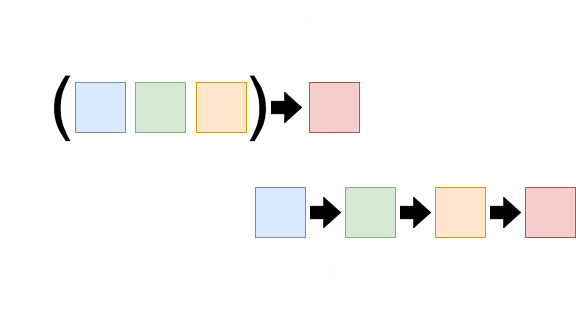
\includegraphics[width=0.5\textwidth]{currying.png}
  \caption{Regularne i Karijeve funkcije}
  \label{fig:currying}
\end{figure}
Strelica (\texttt{\textbf{->}}) je desno asocijativna, a zagrade se izostavljaju zbog
jednostavnosti. Na primer, funkcija \texttt{deljivSa} ima tip \emph{Int -> (Int -> Bool)},
što znači da prihvata vrednost tip \emph{Int} i vraća funkciju tipa \emph{Int -> Bool}.
Karijeve funkcije nam omogućavaju veću fleksibilnost i parcijalnu primenu funkcija, 
odnosno vezivanje argumenata za konkretne vrednosti (listing \ref{listing:tipoviFunkcije}).

\subsubsection{Anotacija tipa funkcije}
Kao što je prethodno prikazano, Elm sam zaključuje tip funkcije, ali dozvoljava i korisniku
da sam navede tip u liniji iznad definicije (listing \ref{listing:anotacija}).
\begin{listing}[!h]
\begin{minted}{haskell}
> deljivSa: Int -> Int -> Bool
| deljivSa x y =
|   modBy x y == 0
|
<function> : Int -> Int -> Bool
\end{minted}
\caption{Anotacija tipa funkcije}
\label{listing:anotacija}
\end{listing}

Korišćenje anotacije tipova nije obavezno, ali je vrlo preporučiljivo iz više razloga.
Prilikom kompilacije proverava se poklapanje anotacije sa stvarnim tipom funkcije, što
dovodi do lakšeg uočavanja i otklanjanja grešaka. Pored toga, anotacije predsavljaju veoma
dobar vid dokumentacije, a činjenica da kompilator uvek poredi navedeni i stvarni tip nam
garantuje da je dokumentacija uvek važeća.

\subsubsection{Funkcijski operatori}
Operatore nad funkcijama možemo podeliti prema tipu, na operatore prosleđivanja i operatore
kompozicije funkcija, i prema smeru u kom se primenjuju, unapred ili unazad.

Operatori prosleđivanja ili \textbf{pipe} operatori su zapravo operatori primene funkcije
i omogućavaju pisanje čitljivijeg koda sa manje zagrada.
\begin{itemize}
  \item \texttt{\textbf{<|}} - pipe operator unazad radi isto što i primene funkcije, 
  s tim što nas oslobađa pisanja zagrada. Preciznije, \texttt{\textbf{ f <| x}} je drugi zapis
  za \texttt{\textbf{ f (x)}}
  \item \texttt{\textbf{|>}} - pipe operator inspirisan je Unix pipe-om, odatle i
  naziv, i služi za prosleđivanje argumenta funkciji. Preciznije,  \texttt{\textbf{ x |> f}}
  je drugi zapis za \texttt{\textbf{ f (x)}}
\end{itemize}

Operator kompozicije unazad \texttt{\textbf{<\smallskip<}} predstavlja operator matematičke 
kompozicije funkcija \(\circ\). Tako da se definicija kompozicije dve funkcije, \((g \circ f)(x) = g(f(x))\),
u Elmu može posmatrati kao: \texttt{\textbf{(g <\smallskip< f) x == (\textbackslash x\textunderscore ->
g ( f x\textunderscore)) x}}. Operator kompozicije \texttt{\textbf{>\smallskip>}} je
simetričan operatoru \texttt{\textbf{<\smallskip<}}, stoga važi: \texttt{\textbf{(f <\smallskip< g) x == (g >\smallskip> f) x}}.

\subsection{Osnovne strukture podataka}
Osnovne strukture podatka u Elmu čine liste, torke i slogovi. 
\subsubsection{Liste}
Lista u Elmu predstavlja kolekciju u obliku jednostruko povezane liste. Elementi se navode
unutar uglastih zagrada---\textbf{\texttt{[\smallskip ]}} i moraju biti istog tipa. Funkcije za rad
sa listama nalaze se unutar \texttt{List} modula, među kojim su i tri veoma važne funkcije 
u funkcionalnoj paradigmi --- \textbf{\texttt{map, filter}} i \textbf{\texttt{fold}} (ili
\textbf{\texttt{reduce}} u drugim programskim jezicima).
Pored operatora za nadovezivanje \textbf{\texttt{++}}, postoji i operator \textbf{\texttt{::}} koji
dodaje element na početak liste, iz istorijskih razloga ovaj operator naziva se kons
(eng. \emph{cons}). 
\begin{listing}[h]
\begin{minted}{haskell}
> "aaa" :: ["bbb","ccc"]
["aaa","bbb","ccc"] : List String
> List.map (List.member 2) [[1,2,3],[2,2],[42]]
[True,True,False] : List Bool
> [1,2]++[3,4,5] |> List.filter (\x -> modBy 2 x == 0) |>List.length
2 : Int
> List.foldl (\x y -> x + y) 0 <| List.range 1 5 
15 : Int
\end{minted}
\caption{Primeri lista različitih tipova i funkcija za rad sa njima}
\label{listing:liste}
\end{listing}
\subsubsection{Torke}
Za razliku od listi koje mogu imati promenljivi broj elemenata istog tipa, torke
predstavljaju kolekcije fiksne dužine čiji elementi ne moraju biti istog tipa.
Mogu sadržati samo dva ili tri elementa, navode se unutar običnih zagrada---
\textbf{\texttt{()}}. U torke se ne mogu ubacivati elementi niti se iz torke mogu
uklanjati elementi. Funkcije nad torkama koje imaju dva elementa nalaze se u modulu
\texttt{Tuple}, dok se za rad sa tokrama od tri elementa koristi poklapanje obrazaca
o kojem će biti više reči kasnije.
\begin{listing}[h]
\begin{minted}{haskell}
> (1,"2",'3')
(1,"2",'3') : ( number, String, Char )
> (1,2) == Tuple.pair 1 2
True : Bool
> Tuple.second ("nebitan", "drugi")
"drugi" : String
> Tuple.mapFirst String.length  ("mapiran", 1)
(7,1) : ( Int, number )
\end{minted}
\caption{Primeri torki i upotreba funkcija iz modula \texttt{Tuple}}
\label{listing:torke}
\end{listing}
\subsubsection{Slogovi} 
Slog (eng. \emph{Record}) predstavlja strukuru podataka koja može sadržati više vrednosti različitih tipova, 
pri čemu je svakoj vrednosti dodeljen naziv. Liče na objekte u JavaScript-u, čak je i 
sintaksa veoma slična, umesto dvotačke slog koristi znak jednakosti za dodelu naziva.
Prilikom definisanja sloga, Elm kreira funkcije za pristup njegovim svojstvima. Nije 
moguće dodavanje, ni uklanjanje svojstava, ali je dozvoljena promena njihovih vrednosti.
Zbog imutabilnosti, ne vrši se promena nad postojećim slogom već se pravi novi.
\begin{listing}[h]
\begin{minted}{haskell}
> pera = {ime = "Pera", prezime = "Perić", godine = 23}
{ godine = 23, ime = "Pera", prezime = "Perić" } 
  : { godine : number, ime : String, prezime : String }
> {pera | prezime = "Petrović", godine = 24}
{ godine = 24, ime = "Pera", prezime = "Petrović" }
  : { godine : number, ime : String, prezime : String }
> pera.ime
"Pera" : String
> .godine pera
23 : number
> .prezime
<function> : { b | prezime : a } -> a
\end{minted}
\caption{Primeri pristupa i promene svojstava sloga}
\label{listing:rekord}
\end{listing}

Pored navedenih struktura podataka, Elm pruža podršku za rad sa nizovima (\texttt{Array}),
skupovima (\texttt{Set}) i rečnicima (\texttt{Dict}).

\subsection{Tipske promenljive} 
U listingu \ref{listing:rekord} vidimo da funkcija za pristup prezimenu ima tip:\\ 
\texttt{\textbf{\{ b | prezime : a \} -> a}}. Ovo znači da funkcija kao argumenat
prima slog, koji može biti bilo kog tipa, ali mora imati svojstvo\texttt{\textbf{
prezime}}, koje takođe može biti bilo kog tipa, i čiji tip je ujedno povrati tip 
funkcije. Promenljive \texttt{\textbf{a}} i \texttt{\textbf{b}} nazivaju se 
\emph{tipske promenljive}, a prisustvo dve tipske promenljive nam govori da one mogu, 
ali ne moraju, predstavljati različite tipove. U konkretnom primeru \texttt{\textbf{a}}
i \texttt{\textbf{b}} su uvek različitog tipa, dok u slučaju funckije \texttt{Tuple.pair
: a -> b -> ( a, b )} mogu biti istog tipa. Prilikom anotacije tipova mogu se koristi i
duža imena tipskih pormenljivih, a pravlia imenovanja su ista kao i za funkcije.

Tipske promenljive u Elmu ukazuju na prisustvo \textbf{parametarskog polimorfizma},
jedine vrste polimorfizma u ovom jeziku.

\subsubsection{Uslovne tipske promenljive}
Za razliku od Haskell-a, sistem tipova u Elmu nije toliko složen i umesto tipskih 
klasa (eng. \emph{typeclasses})\cite{typeclasses} poseduje jednostavniji koncept
---\emph{uslovne tipske promenljive}. 

Uslovne tipske promenljive omogućavaju da se na određni način ograniči skup tipova
koji se može koristiti u izrazima. Najčešći primer je \texttt{number}, koji dozvoljava 
isključivo \texttt{Int} ili \texttt{Float} tipve. 

U trenutnoj verziji (\emph{0.19.1}) postoje četiri uslovne tipske promenljive:
\begin{enumerate}
  \item \texttt{number} --- dozvoljava tipove \texttt{Int} i \texttt{Float}
  \item \texttt{appendable} --- dozvoljava tipove \texttt{String} i \texttt{List a}
  \item \texttt{comparable} --- dozvoljava tipove \texttt{Int}, \texttt{Float}, \texttt{Char},
  \texttt{String}, liste i torke koje sadrže \texttt{comparable} vrednosti
  \item \texttt{compappend} --- dozvoljava tipove \texttt{String} i \texttt{List comparable}
\end{enumerate}

\subsubsection{Operatori i tipske promenljive}
\begin{listing}[h]
\begin{minted}{haskell}
> (+) 1 2
3 : number
> (*)
<function> : number -> number -> number
> (++)
<function> : appendable -> appendable -> appendable
> (==)
<function> : a -> a -> Bool
> (>=)
<function> : comparable -> comparable -> Bool
\end{minted}
\caption{Upotreba operatora u prefiksnoj notaciji}
\label{listing:tipskePromenljive}
\end{listing}
Operatori u Elmu predstavljaju funkcije koje se mogu pozivati u infiksnoj notaciji. Takođe, 
mogu se pozivati i u prefiksnoj ukoliko ih navedemo unutar zagrada: \texttt{\textbf{(+),
(++), (>=)}}... , dok pozivanjem bez argumenata možemo videti i kog su tipa (listing \ref{listing:tipskePromenljive}).

U ranijim verzijama jezika bilo je moguće definisati korisničke operatore, ali je ta
opcija izbačena u verziji 0.19.0., a od verziji 0.18.0 nije moguće pozivanja 
binarnih funkcija u infiksnoj notaciji.

\subsection{Alijasi tipova}
Prilikom definisanja funkcija koje rade nad istim strukturama podataka višestruko navodimo
iste anotacije tipova, pritom anotacije podataka mogu biti predugačke, samim tim i
teško čitljive. Alijasi tipova nam omogućavaju ponovnu upotrebu anotacija i bolju čitljivost.
Definišu se pomoću ključnih reči \texttt{\textbf{type alias}}, nakon kojih sledi ime koje
mora počinjati velikim slovom. 
\begin{listing}[h]
\begin{minted}{haskell}
>type alias MatricaInt3 = List (List (List Int))
>
>type alias Osoba = {ime : String, prezime : String, godine : Int }
> Osoba
<function> : String -> String -> Int -> Osoba
> Osoba "Pera" "Perić" 23
{ godine = 23, ime = "Pera", prezime = "Perić" } : Osoba
\end{minted}
\caption{Primeri definisanja alijasa tipova}
\label{listing:alias}
\end{listing}

Prilikom kreiranja alijasa za slog kreira se i konstruktor za slog, što se može videti
u listingu \ref{listing:alias}. Redosled argumenata funkcije za konstrukciju identičan je
redosledu u alijasu.
\subsection{Korisnički definisani tipovi}
Pored korišćenja alijasa za postojeće tipove podataka, Elm pruža mogućnost kreiranja novih 
tipova. Korisnički definisani tipovi se često nazivaju i \emph{unijski tipovi}, jer mogu  
predstavljati uniju više varijanti definisanog tipa. Definišu se ključnom reči 
\textbf{\texttt{type}}, a varijante se odvajaju simbolom \texttt{\textbf{|}}.

Slično kao kod alijasa tipova za slogove i ovde se kreiraju konstruktori za definisani tip. 
\begin{listing}[h]
\begin{minted}{haskell}
> type VectorF4 = Vector4F Float Float Float Float
> Vector4F
<function> : Float -> Float -> Float -> Float -> VectorF4
>
>type StatusPrijave 
  = NaCekanju 
  | Greska String 
  | Uspesno {id : Int, token : String}
> NaCekanju
NaCekanju : StatusPrijave
> Greska
<function> : String -> StatusPrijave
> Uspesno
<function> : { id : Int, token : String } -> StatusPrijave
\end{minted}
\caption{ Primeri korisnički definisanih tipova}
\end{listing}

\subsection{Kontorla toka}
U Elmu nema izvršavanja naredbi, već samo evaluacije izraza, tako da umesto naredbi grananja
imamo izraze \texttt{\textbf{if}} i \texttt{\textbf{case}}, a rekurziju umesto petlji.  
\subsubsection{Izraz \texttt{\textbf{if}}}
Izraz \texttt{\textbf{if}} se može posmatrati kao ternarni operator u JavaScript-u, C++-u i 
mnogim drugim programskim jezicima.
\begin{listing}[h]
\begin{minted}{haskell}
{-    uslov   ?  izraz1   :  izraz2   - ternarni operator
   if uslov then izraz1 else izraz2   - if izraz
-}
if x >= 0 then "pozitivan" else "negativan"
if x == 1 then x * 2 else if x == 2 then x / 2 else x
\end{minted}
\caption{Sintaksa izraz \texttt{\textbf{if}} i primer upotrebe}
\label{listing:if}
\end{listing}

Ključna reč \texttt{\textbf{else}} je sastavni deo izraza \texttt{\textbf{if}} tako
da \texttt{\textbf{else}} "grana" uvek postoji. Mogu se navoditi i ugnježdeni
izrazi \texttt{\textbf{if}}, pa \texttt{\textbf{else if}} grana predstavlja korišćenje
izraza \texttt{\textbf{if}} nakon ključna reč \texttt{\textbf{else}}.

\subsubsection{Izraz \texttt{\textbf{case}}}
Izraz \texttt{\textbf{case}} predstavlja pandan \texttt{\textbf{switch}} naredbi u drugim
programski jezicima. Prilikom korišćenja izraza \texttt{\textbf{case}} moraju se pokriti sve
mogućnosti, ukoliko to nije slučaj kompilator prijavljuje grešku. Za podrazumevani slučaj
može se korisiti simbol \texttt{\textbf{\textunderscore}}. Izraz \texttt{\textbf{case}}
zauzima značajno mesto u Elmu, jer se koriste u \textbf{poklapanju obrazaca}.
\begin{listing}[h]
\begin{minted}{haskell}
case mesto of
  1 -> "zlato"
  2 -> "srebro"
  3 -> "bronza"
  _ -> "zahvalnica"
\end{minted}
\caption{Primer upotrebe izraza \texttt{\textbf{case}}}
\label{listing:case}
\end{listing}
\subsubsection{Izraz \texttt{\textbf{let}}}
Budući da ne postoje blokovi naredbi, izrazi \texttt{\textbf{let}} nam omogućavaju da 
ograničimo oblast važenja --- dosega (eng. \emph{scope)} funkcija i konstanti u okviru
jedne funkcije. Doprinose boljoj čitljivosti koda, a moguće je koristiti anotacije tipova
unutar njih.
\begin{listing}[h]
\begin{minted}{haskell}
let
  nula: Int
  nula = 0
  
  pozitivan: Int -> Bool
  pozitivan =
    \x -> x > nula
in pozitivan 10
\end{minted}
\caption{Primer upotrebe izraza \texttt{\textbf{let}}}
\end{listing}
\subsubsection{Rekurzija}
Rekurzivno definisana funkcija poziva samu sebe, čime se postiže ponavljanje izvršavanja
koje se u imperativnom programiranju ostvaruje korišćenjem petlji. U mnogim slučajevima,
umesto rekurzije mogu se koristiti funkcije nad listama.
\begin{listing}[h]
\begin{minted}{haskell}
factorial n = 
  if n <= 1 then 1 
  else  n * factorial (n - 1)

factorialFold n = 
  List.foldl (*) 1 (List.range 1 n) 
\end{minted}
\caption{Upotreba rekurzije i \texttt{foldl} funkcije za iteraciju kroz listu}
\end{listing}

\subsection{Poklapanje obrazaca}
Poklapanje obrazaca može se posmatrati kao pokušavanje usklađivanja (poklapanja) ulaznog
podatka sa unapred definisanim obrascom. Ukoliko dođe do usklađivanja, poklopljenim
vrednostima se može prisupiti putem identifikatora definisanim u obrascu. Pored spomenutih
\texttt{\textbf{case}} izraza, u Elmu se poklapanje obrazaca može korisiti u vidu 
razlaganja slogova ili torki prilikom definisanja funkcija ili korišćenja\texttt{\textbf{
let}} izraza.
\begin{listing}[h]
\begin{minted}{haskell}
-- liste 
case lista of
  [] -> "prazna lista"
  [_] -> "jedan element"
  [a,b] -> "dva elementa:" ++ a ++ " i " ++ b
  a :: _ -> "više od dve elemenata, prvi je: " ++ a

-- unijski tipovi
case prijava of
  NaCekanju -> "Molimo za strpljejne"
  Greska poruka -> "Došlo je do grške: " ++ poruka
  Uspesno {id} -> "Uspešna prijava, id: " ++ String.fromInt id

-- torke
case tacka3D of
  (0, 0, 0) -> "centar"
  (0, _, _) -> "na x-osi"
  _ -> "van x-ose"

-- razlaganje
let
  (x,_,_) = tacka3D
in "x koordinata je " ++ String.fromFloat x

--nije moguće poklapanje ugnježdenih slogova
prikaziPodatke ({ime, adresa} as osoba) =
  ime ++ " " ++ osoba.prezime ++ " " ++ adresa.ulica
\end{minted}
\caption{Primeri poklapanja obrazaca}
\label{listing:pokalapanjeObrazaca}
\end{listing}

Unutar case izraza sekvencijalno se vrši poklapanje obrazaca. Kada dođe do poklapanja
izračunava se izraz dodeljen datom obrascu, ne nastavlja se sa poklapanjem. Kompilator
prepoznaje ukoliko može doći do nepoklapanja nijednog obrasca i prijavljuje grešku.
Takođe, greška se prijavljuje i ukoliko se navede redudantan obrazac, tj. obrazac čiji je
skup vrednosti zapravo podskup skup vrednosti prethodno definisanog obrasca. 
Simbol \texttt{\textbf{\textunderscore}} služi za poklapanje vrednosti koje se ne koriste,
a ključna reč \texttt{\textbf{as}} se može koristiti ukoliko je potrebno pristupiti celom
ulaznom podatku. U listingu \ref{listing:pokalapanjeObrazaca} mogu se videti primeri
poklapanja obrazaca.

\subsection{Obrada grešaka pomoću \texttt{\textbf{Maybe}} i \texttt{\textbf{Result}}}
U Elmu ne postoje \texttt{\textbf{try catch}} blokovi, kao ni \texttt{\textbf{undefined, null, nil}}
i ostale slične vrednost prisutne u drugim programskim jezicima.
Umesto njih koriste se \texttt{\textbf{Maybe}} i \texttt{\textbf{Result}} koji potiču iz Haskell-a,
gde imamo \texttt{\textbf{Maybe}} i \texttt{\textbf{Either}}.

\subsubsection{Maybe}
U slučaju da je potrebno napisati funkciju koja vraća prvi element liste, ukoliko on
postoji, rezultat bi bio \textbf{baš} prvi element. Dok u slučaju prazne liste, funkija ne
bi vratila \textbf{ništa}. Upravo tako radi funkcija \texttt{List.head : List a -> Maybe a}, 
ukoliko se pozove \textbf{možda} vrati prvi element.

\texttt{\textbf{Maybe}} se definiše kao \texttt{\textbf{type Maybe a = Just a | Nothing}}
i može se koristiti za opcione argument, obradu grešaka i u slogovima sa opcionim svojstvima.
Zapravo svuda gde očekivani podatak može, ali ne mora, postojati.

\subsubsection{Result}
Za razliku od \texttt{\textbf{Maybe}}, koji bi u slučaju greške vratio \texttt{
\textbf{Nothing}}, \texttt{\textbf{Result}} nam daje mogućnost pružanja dodatnih 
informacija o grešci. Definiše se na sledeći način: \begin{tabbing}
\texttt{\textbf{type}} \= \texttt{\textbf{ Result error value}} \\
\> \=  \texttt{\textbf{= Ok value}} \\\>
\> \texttt{\textbf{| Err error }}
\end{tabbing}

\section{Arhitektura Elm}
Arhitektura Elm je veoma jednostavan obrazac projektovanja veb aplikacija koji se pojavljuje
ubrzo nakon nastanka samog jezika Elm. Nastaje prirodno, tako što rani Elm programeri uočavaju
iste obrase u svom kodu, koji se mogu podeliti u tri dela:
\begin{enumerate}
  \item Model - stanje aplikacije
  \item Pogled (eng. \emph{View}) - transormacija stanja u HTML
  \item Ažuriranje (eng. \emph{Update}) - promena stanja
\end{enumerate}
\begin{figure}[!ht]
\centering
\begin{subfigure}{.5\textwidth}
  \centering
  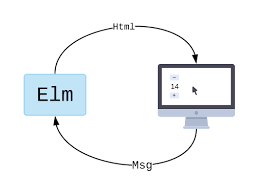
\includegraphics[width=.8\linewidth]{elm-arch-site}
\end{subfigure}%
\begin{subfigure}{.5\textwidth}
  \centering
  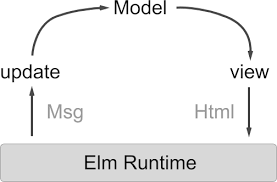
\includegraphics[width=.7\linewidth]{elm-arch-book}
\end{subfigure}
\caption{Elm arhitektura}
\label{fig:elm-arh}
\end{figure}

U levom delu slike \ref{fig:elm-arh} prikazano je kako radi svaki Elm program: generiše
se HTML koji se prikazuje u pretraživaču, nakon čega pretraživač šalje poruku programu
ukoliko se nešto dogodilo. U desnom delu slike vidimo šta se dešava unutar programa,
na osnovu primljene poruke funkcija \texttt{\textbf{update}} kreira novi\texttt{
\textbf{model}}, koji se prosleđuje funkciji \texttt{\textbf{view}}, na osnovu koje
se generiše HTML.

Ovaj obrazac projektovanja ce često naziva i MVU (eng. \emph{Model-View-Update}). Za 
razliku od obrazaca MVC \cite{jsPatterns} (eng.\emph{Model-View-Controller}) i MVVM \cite{jsPatterns}
(eng. \emph{Model-View-ViewModel}), koji stanje aplikacije dele na više manjih modela,
u Elm arhitekturi celokupno stanje apikacije se nalazi na jednom mestu, tj. modelu, a
protok podataka kroz aplikaciju je uvek u jednom smeru. 

Arhtitektura Elm uticala je na nastajanje velikog broja biblioteka za upravljanje
stanja veb aplikacija, među kojima su najpoznatije Redux\cite{redux} i Vuex\cite{vuex}.
Takođe, podrška za rad sa MVU obrascem počinje da se pojavljuje i u drugim tehnologijama,
jedna od njih je i .NET 5 \cite{net5}.

\subsection{Generisanje HTML sadržaja}
Za razliku od drugih radnih okruženja koji uglavnom koriste HTML šablone, Elm za 
opisivanje izgleda stanice koristi funkcije. Stoga imamo funkcije za kreiranje HTML
čvorova i atributa.
\begin{listing}[h]
  \begin{minted}{haskell}
  --   <button   id="btn-ok"  class="btn-default">    Ok      <\button>
  node "button" [id "btn-ok", class "btn-default"] [text "Ok"]
  -- korišćenje pomoćne funkcije button umesto node "button"
        button  [id "btn-ok", class "btn-default"] [text "Ok"]
  \end{minted}
  \caption{Primeri kreiranje HTML čvorova}
  \label{listing:nodeHtml}
  \end{listing}
  
Funkcija \texttt{\textbf{node}} iz modula \texttt{\textbf{Html}} predstavlja generičku
funkcija za kreiranje HTML čvorova, koja kao argumente prima HTML oznaku, listu atributa
i listu čvorova (deca čvora). U listingu \ref{listing:nodeHtml} predstavljena je analogija
kreiranja HTML čvora funkcijom \texttt{\textbf{node}} i HTML sintakse.
Modul \texttt{\textbf{Html}} pruža veliki broj pomoćnih funckija, koje imaju nazive po
HTML oznakama (npr. \texttt{\textbf{button}} --- listing \ref{listing:nodeHtml}) i omogućavaju bolju čitljivost. Stoga se 
funkcija \texttt{\textbf{node}} koristi prilikom upotrebe korisnički definisanih elemenata
ili ukoliko ne postoji pomoćna funkcija za željeni element. Funkcija \texttt{\textbf{text}}
služi za postavljanje teksta u DOM, dok su \texttt{\textbf{id}} i \texttt{\textbf{class}}
funkcije za kreiranje atributa iz modula \texttt{\textbf{Html.Attributes}}.

\subsection{Elm program}
Prilikom inicijalizacije Elm projekta se, pored paketa \texttt{\textbf{elm/core}} sa
osnovnim funkcionalnostima i strukturama podataka i paketa \texttt{\textbf{elm/html}} za
generisanje HTML stranica, nalazi paket \texttt{\textbf{elm/browser}} za kreiranje Elm
programa u pretraživaču. Unutar ovog paketa, u modulu \texttt{\textbf{Browser}} se nalaze
funkcije koje nam omogučavaju kreiranje različitih tipova programa, među kojima je i
funkcija \texttt{\textbf{sandbox}} namenjena za učenje osnova Elm arhitekture i
omogućava bazičnu interakciju sa korisnicima, bez komunikacije sa spoljnim svetom.
Primer jednostavanog Elm programa upotrebom \texttt{\textbf{sandbox}} funkcije prikazan
je u listingu \ref{listing:elmProgram}.
\begin{listing}[h!]
\begin{minted}{haskell}
  module Main exposing (main)

  import Browser
  import Html exposing (Html, button, div, text)
  import Html.Events exposing (onClick)
  
  main =
    Browser.sandbox { init = init, update = update, view = view }

  --MODEL
  type alias Model = Int
  
  init : Model
  init =
    0
  
  -- UPDATE
  type Msg
    = Increment
    | Decrement
  
  update : Msg -> Model -> Model
  update msg model =
    case msg of
      Increment ->
        model + 1
  
      Decrement ->
        model - 1
  
  -- VIEW
  view : Model -> Html Msg
  view model =
    div []
      [ button [ onClick Decrement ] [ text "-" ]
      , div [] [ text (String.fromInt model) ]
      , button [ onClick Increment ] [ text "+" ]
      ]
\end{minted}
\caption{Primer Elm programa}
\label{listing:elmProgram}
\end{listing}

Da bi Elm okruženje znalo koja je polazna tačka programa potrebno je da se u glavnom
modulu definiše i izloži konstanta \textbf{\texttt{main}}, dok naziv modula nije bitan.
Pored funkcija iz modula \texttt{\textbf{Browser}}, u slučaju statičkih stranica, konstanta 
\textbf{\texttt{main}} se može definistati funkcijama iz modula \texttt{\textbf{Html}},
na primer: \mint{haskell}|main = text "Zdravo svete!"|

Da bi se pokrenuo program potrebno je pozicionirati se u komandnoj liniji na inicijalizovani
Elm projekat i pokrenuti \texttt{\textbf{elm reactor}}. Nakon toga, potrebno je otvoriti pretraživač na
adresi \emph{http://localhost:8000} i unutar \texttt{\textbf{src}} direktorijuma kliknuti na 
\texttt{\textbf{Main.elm}} čime se vrši kompilacija i pokretanje programa. Takođe, primer se
može naći i na zvaničnom Elm vodiču\cite{elm-program}.

U primeru jednostavnog brojača iz listinga \ref{listing:elmProgram} vidimo da funkcija
\textbf{\texttt{sandbox}} kao argument prima slog sa inicijalnom vrednošću modela i 
funkcijama za ažuriranje i prikazivanje modela. Program počinje sa pozivanjem funkcije
\texttt{\textbf{view}} sa parametrom \texttt{\textbf{init}}. Unutar funkcije
\texttt{\textbf{view}} se pomoću funkcije za kreiranje atributa iz modula
\texttt{\textbf{Html.Events}} mogu definisati načini slanja poruka, a kao rezultat 
izvršavanja nastaje virtuelni DOM, na osnovu kog Elm okruženje izmenjuje stvarni DOM.
Ukoliko dođe do odgovarajuće akcije korisnika, u ovom sličaju klikom na dugme, Elm okruženje
generiše poruku i prosleđuje je zajedno sa modelom funkciji \texttt{\textbf{update}} koja
kreira novi model nad kojim se poziva ponovo funkcija \texttt{\textbf{view}}.
Elm okruženje poredi prethodni virtuelni DOM sa novim i vrši minimalan broj izmena.  

\chapter{Elixir}
Osnovne odlike jezika Elixir sažete su u okviru njegove zvanične strane \cite{elixir}:
\begin{displayquote}
Elixir je dinamički tipiziran, funkcionlni programski jezik dizajniran za izgradnju skalabilnih
aplikacija, lakih za održavanje.

Elixir koristi virtuelnu mašinu programskog jezika Erlang, poznatu po podršci za rad sistema sa malim kašnjenjem,
distribuiranim sistemima i sistemima otpornim na greške, takođe se uspešno koristi u razvoju
veba, u sistemima sa ugrađenim računarom (eng. \emph{embedded sotfware}), učitavanju podataka
(eng. \emph{data ingestion}) i u domenima za obradu mulitmedije.
\end{displayquote}

Prva verzija programskog jezika Elixir objavljena je 2011. godine. Autor jezika, Žozé Valim
(José Valim), prethodno je radio kao \emph{Ruby} programer i uvideo je probleme rada \emph{Ruby
on Rails} okruženja na višejezgarnim sistemima. Rešenje problema video je u novom funkcionalnom
programskom jeziku koji će koristiti prednosti virtuelne mašine jezika Erlang. Stoga, najveći
uticaj na razvoj programskog jezika Elixir imali su Erlang, sa kojim je semantički vrlo sličnan,
i Ruby u smislu sintakse. 

Ruby je dinamički tipiziran programski jezik opšte namene koji pruža mogućnost rada u više
programskih paradigmi. Nastao je sredinom devedesetih godina prošlog veka, a razvio ga je 
japanski naučnik i programer Jukihiro Macumoto (Yukihiro Matsumoto). Ruby je dizajniran
kao programski jezik fokusiran na programera, tako da svojom lakoćom korišćenja, jednostavnošću i 
fleksibilnošću učini programiranje prijatnijim. Sam autor kaže da pokušava da napravi Ruby 
što prirodnijim.  

Budući da je Elixir nastao na ideji upotrebe virtuelne mašine jezika Erlang, više o Erlang-u biće rečeno
u sledećem poglavlju. Takođe, pored dva navedena programska jezika, uticaj na razvoj Elixir-a 
imali su Clojure\cite{clojure}, Haskell\cite{haskell} i Python\cite{python}.

\section{Erlang}
Erlang nije samo programski jezik, već i razvojna platforma za izgradnju skalabilnih i pouzdanih
sistema koji gotovo neprestano pružaju usluge. Švedske telekomunikaciona kompanija Erikson (eng.
\emph{Ericsson}) osmislila je ovu platformu sredinom  osamdesetih godina prošlog veka. 
Da bi Erlang mogao da upravlja telekomunikacionim sistemima kompanije, morao
je da bude pouzdan, skalabilan, da ima brz odziv i bude konstantno dostupan, jer telefonska mreža
mora da funkcioniše bez obzira na broj istovremenih poziva, neočekivane grešake ili hardver.

Iako je prvobitno izgrađen za telekomunikacione sisteme, Erlang ni na koji način nije 
specijalizovan za ovaj domen, ne sadrži podršku za programiranje telefona i drugih 
telekomunikacionih uređaja. Erlang predstavlja razvojnu platforma koja pruža posebnu podršku
tehničkim, nefunkcionalnim zahtevima kao što su: paralelnost, skalabilnost, tolerancija na
greške, distribuiranost i velika dostupnost. U vreme njegovog nastajanja, programi su se uglavnom
koristili bez komunikacije sa nekim veb servisom (eng. \emph{desktop-based sotfware}), pa je 
upotreba Erlang-a bila ograničena na telekomunikacione sisteme. Međutim, zahtevi modernih 
sistema i aplikacija poklapaju se sa nefunkcionalnim zahtevima za koje Erlang pruža podršku, tako
da je u poslednje vreme privukao veliku pažnju. Erlang pokreće razne velike sisteme, među kojima
su aplikacije \emph{WhatsApp}\cite{whatsapp} i \emph{WeChat}\cite{wechat}, \emph{Riak}\cite{riak}  
distribuirana baza podataka i \emph{Heroku Cloud}\cite{heroku}.

Kao razvojna platforma, Erlang se sastoji od jezika, virtuelne mašine, razvojnog okvira (eng.
\emph{framework}) i alata.
\subsection{Erlang virtuelna mašina --- BEAM}
Jezik Erlang predstavlja primaran način pisanja koda koji se izvršava na sopstvenoj virtuelnoj
mašini koja se naziva BEAM. BEAM je skraćenica za \emph{Bogdan’s Erlang Abstract Machine}, po
Bogumilu Bogdanu Hausmanu koji je kreirao originalnu verziju, ali se može posmatrati i kao
\emph{Björn’s Erlang Abstract Machine}, po Bjornu Gustavsonu koji održava trenutnu verziju 
virtuelne mašine. 

K\^{o}d napisan u Erlang-u se prevodi u binarni k\^{o}d (eng. \emph{bytecode})
koji se unutar BEAM-a izvršava paralelno u vidu veoma lakih \emph{Erlang procesa}. BEAM, umesto 
da se oslanja na procese i niti operativnog sistema, samostalno raspoređuje konkurente
\emph{Erlang procese} na dostupna procesorska jezgra, što je prikazano na slici \ref{fig:beam}.
\begin{figure}[h]
  \centering
  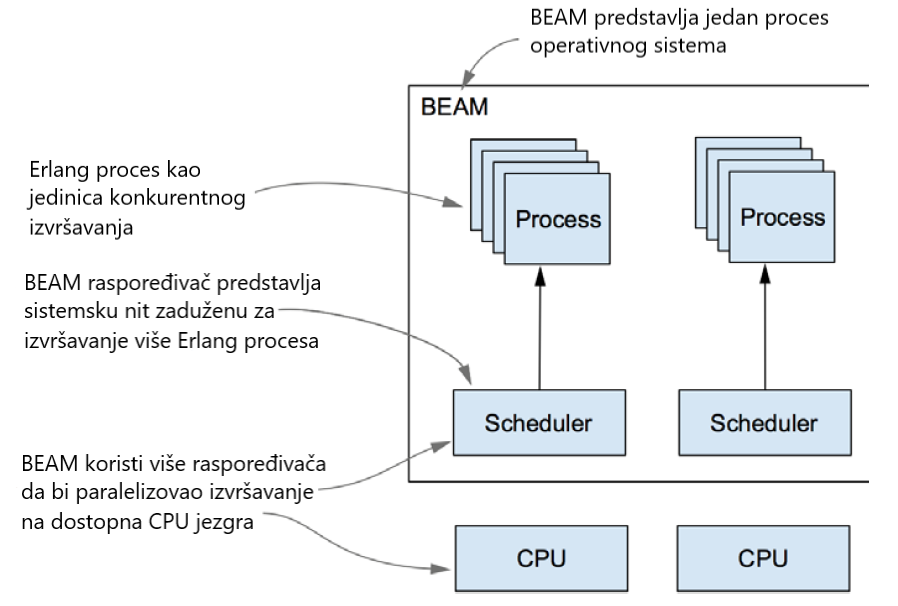
\includegraphics[width=0.6\textwidth]{beam.png}
  \caption{Način izvršavanja Erlang procesa unutar BEAM-a \cite{elixirInAction}}
  \label{fig:beam}
\end{figure}
Ovi laki procesi su međusobno potpuno izolovani, ne dele memoriju i komuniciraju preko
asinhronih poruka, što pruža mogućnost Erlang sistemima da budu skalabilni, distribuirani i 
otporni na greške.  

\subsection{OTP razvojni okvir}
OTP je skraćenica za \emph{Open Telecom Platform}, što je donekle pogrešan naziv za ovaj razvojni
okvir. On nije vezan za telekom sisteme, već predstavlja razvojni okvir opšte namene koji
apstrahuje tipične zadatke Erlang sistema:
\begin{itemize}
  \item Obrasce konkurentnosti i distribuiranosti
  \item Detekciju i oporavak od grešaka u konkurentim sistemima
  \item Pravljanje biblioteka
  \item Postavljanje (eng. \emph{deployment}) sistema
  \item Uživo ažuriranje softvera 
\end{itemize}
OTP predstavlja sastavni deo Erlang-a, stoga i zvanična distribucija nosi naziv Erlang/OTP.
\subsection{Erlang i Elixir}
Elixir predstavlja alternativni načina pisanja programa koji se izvršava na BEAM virtuelnoj
mašini i samim tim preuzima sve osobine Erlang platforme. Za razliku od Erlang-a pruža dodatne
koncepte koji omogućavaju značajno smanjenje ponavljajućeg i šablonskog (eng.
\emph{boilerplate}) koda. Elixir i Erlang su kompatibilni, pa Elixir može direktno da koristi
Erlang biblioteke i module. Važi i obrnuto, a sve što je moguće implementrati u Erlang-u,
moguće je i u Elixir-u bez razlike u performansama. Takođe, važno je napomenuti da oba jezika
odlikuje nepromenljivost podataka (imutabilnost).
\section{Osnovne karakterisike jezika Elixir}
Za razliku od Elm-a, Elixir nije čist funkcionalni programski jezik, jer dozvoljava bočne efekte.
Pored prethodno spomenutih karakteristika preuzetih od Erlang-a, dinamičke tipiziranosti i 
sintakse slične Ruby-ju, Elixir odlikuje izraženo poklapanje obrazaca, polimorfizam, makroi
i metaprogramiranje, kao i podrška za lenjo izračunavanje.   
\section{Uputstvo za instalaciju}
Proces instalacije je vrlo jednostavan, potrebno je pratiti uputstva sa zvanične Elixir
stranice \cite{elixir} za odgovarajući operativni sistem. Podržani su gotovo svi operatini
sistemi. Provera usprešne instalacije može se izvršiti pokretanjem komande
\textbf{\texttt{elixir -{}-version}} u komandnoj liniji ili pokretanjem interaktivnog Elixir-a
komandom \textbf{\texttt{iex}}.

\section{Osnovni tipovi podataka}
Osnovni tipovi podataka u Elixir-u predstavljaju brojevi (celobrojni i realni), bulovske
vrednosti, atomi i stringovi. Takođe, u osnovne tipove podataka jezika Elixir ubrajaju se liste i torke. Pregled
osnovnih tipova dat je u listingu \ref{listing:tipoviElixir}, gde se može videti i način pisanja
komentara. Elixir podržava samo linijske komentare koji se označavaju simbolom \texttt{\textbf{\#}}.
\begin{listing}[!h]
\begin{minted}{elixir}
iex> 1          # integer
iex> 1.0        # float
iex> true       # boolean 
iex> :atom      # atom
iex> "elixir"   # string
iex> [1, 2, 3]  # lista
iex> {1, 2, 3}  # torka
\end{minted}
\caption{Pregled osnovnih tipova podataka u Elixir-u}
\label{listing:tipoviElixir}
\end{listing}

\subsection{Celi brojevi}
Za razliku od Elm-a, celi brojevi u Elixir-u nemaju ograničen opseg vrednosti. Takođe, pored
heksadecimalnog zapisa, Elixir pruža mogućnost navođenja celobrojnih vrednosti u binarnom i 
oktalnom obliku. Simbol \texttt{\textbf{\textunderscore}} može se koristiti za odvajanje 
cifara i kod celih i kod brojeva u pokretnom zarezu (listing \ref{listing:brojeviElixir}).
\subsection{Brojevi u pokretnom zarezu}
Brojevi u pokretnom zarezu su dvostruke preciznosti (64 bita) po standardu \emph{IEEE-754}.
Vrednosti se mogu navoditi i u eksponencijalnom zapisu, a za razliku od Elm-a ne postoje 
vrednost kao što su \texttt{NaN} ili \texttt{Infinity}.
\begin{listing}[!h]
\begin{minted}{elixir}
iex> 10_000
10000
iex> 0o77
63
iex> 0b111_111
63
iex> 0xFF
255
iex> 1_000_000.000_123
1000000.000123
iex> 1.23e-3
0.00123
\end{minted}
\caption{Primeri celih i realnih brojeva u Elixir-u}
\label{listing:brojeviElixir}
\end{listing}
\subsection{Atomi}
Atom je konstanta čiju vrednost predstavlja njeno ime. Definiše se dvotačkom (\texttt{\textbf{:}}),
nakon koje slede alfanumerički karakteri, simboli \texttt{\textbf{@}} ili 
\texttt{\textbf{\textunderscore}}, a može se završavati znakom pitanja ili uzvika. Takođe, moguće
je koristite i razmake, tada se sadržaj posle dvotačke mora navesti unutar navodnika.
Postoji i notacija atoma bez početne dvotačke, ali u tom slučaju moraju počinjati velikim
slovom i takvi atomi se nazivaju \emph{alijasi}. Upotreba atoma prikazana je u listingu
\ref{listing:atomi}.

Atom se sastoji od teksta i vrednosti. U toku izvršavanja tekst se čuva u \emph{tabeli atoma},
dok vrednost predstavlja referencu na tekst u tabeli atoma, što omogućava brže poređenje atoma
kao i veću uštedu memorije. Obzirom da predstavljaju efikasan način za imenovanje konstanti,
atomi su svuda prisutni.
\begin{listing}[!h]
\begin{minted}{elixir}
iex> :neka_vrednost
:neka_vrednost
iex> :"atom sa razmacima"
:"atom sa razmacima"
iex> AliasAtom # tokom kompilacije se transformiše u :"Elixir.AliasAtom"
AliasAtom
iex> AliasAtom == :"Elixir.AliasAtom"
true
\end{minted}
\caption{Primeri atoma u Elixir-u}
\label{listing:atomi}
\end{listing}
\subsubsection{Bulovske vrednosti kao atomi}
Elixir zapravo nema poseban tip za bulovske vrednosti, već koristi atome \texttt{\textbf{:true}}
i \texttt{\textbf{:false}}, i pruža mogućnost njihovog navođenja bez početne dvotačke. U okviru
modula \texttt{Kernel}, koji predstavlja pandan modulu \texttt{Basics} u Elm-u, Elixir pruža
funkcije za proveru tipa, među kojima su \texttt{\textbf{is{\textunderscore}atom}} i
\texttt{\textbf{is{\textunderscore}boolean}} i čija upotreba je predstavljena u listingu
\ref{listing:boolAtomi}.
\begin{listing}[!h]
\begin{minted}{elixir}
iex> is_atom(true)
true
iex> is_boolean(:true)
true
iex> false == :false
true
\end{minted}
\caption{Predstavljanje bulovskih vrednosti preko atoma}
\label{listing:boolAtomi}
\end{listing}

Pored bulovskih vrednosti, jos jedna specifična vrednost predstavljena atomom jeste
\texttt{\textbf{:nil}}, slična vrednosti \texttt{\textbf{null}} u drugim programskim jezicima.
Ona se takođe može navoditi bez početne dvotačke.
\subsection{Stringovi}
Stringovi se navode identično kao u Elm-u, unutar jednostrukih ili trostrukih navodnika. 
U Elixir-u, stringovi koriste UTF-8 kodiranje i pružaju mogućnost ugrađivanja izraza --- interpolaciju
stringova, što se može videti u listingu \ref{listing:elixirString}. Modul \texttt{Kernel}
pruža operator konkatenacije (\texttt{\textbf{<>}}), a funkcije za rad sa stringovima nalaze
se u modulu \texttt{String}.
\begin{listing}[!h]
\begin{minted}{elixir}
iex> "Ćao!"
"Ćao!"
iex> "1+1=#{1+1}"
"1+1=2"
iex> "primer " <> "konkatenacije"
"primer konkatenacije"
iex> String.length("Ćao")
3
\end{minted}
\caption{Primeri stringova u Elixir-u}
\label{listing:elixirString}
\end{listing}
\subsubsection{Bitstringovi i sekvence bajtova}
Kao i kod bulovskih vrednosti, Elixir nema poseban tip za stringove, već za njihovo
predstavljanje koristi sekvencu bajtova (eng. \emph{binary}) i UTF-8 kodiranje.
Zapravo fundamentalni tip za njihovo predstaljanje jeste \textbf{bitstring}, kojem odgovara 
neprekidni niz bitova u memoriji. Bitstringovi mogu biti proizvoljne dužine, a sekvenca
bajtova ---\emph{binary} predstavlja posebnu vrstu bitstringova čiji je broj bitova deljiv sa
osam. 

Bitstringovi se navode kao sekvenca brojeva unutar znakova
\texttt{\textbf{<\smallskip<}} i \texttt{\textbf{>\smallskip>}}. Podrazumevano se koristi
osam bitova za čuvanje svakog broja u bitstringu, ali je moguće navesti broj bitova pomoću
modifikatora \texttt{\textbf{::n}} da bi se oznaćila veličina od \texttt{\textbf{n}} bitova,
ili u opširnijoj notaciji \texttt{\textbf{::size(n)}}.
\begin{listing}[!h]
\begin{minted}{elixir}
iex> is_binary(<<1,2>>)
true
iex> is_bitstring(<<1::1>>) # 1 bit
true
iex> is_binary(<<1::1,2>>) # 9 bitova
false
iex> <<1::1,0::1,1::1>>
<<5::size(3)>>
iex> is_binary("neki string")
true
iex> byte_size("Ćao") # Ć zauzima 2 bajta
4
iex> ?a # određivanje koda karakter a
97
iex> <<97,98,99>>  
"abc"
iex> "123" <> <<0>> # konkatenacija
<<49, 50, 51, 0>>
\end{minted}
\caption{Predstavljane stringova kao niz bajtova}
\label{listing:elixirBitstring}
\end{listing}
U listingu \ref{listing:elixirBitstring} vidimo da je operator \texttt{\textbf{<>}} zapravo
operator kontatenacije bitstringova i ukoliko sadržaj bitstringa čine samo ASCII
karakteri, interaktivni Elxir ispisuje string. Elixir nema tip \texttt{Char} za rad sa
karakterima, ali daje mogućnost određivanja koda pomoću simbola \texttt{\textbf{?}}, nakon 
kog se navodi karakter. 

\subsection{Liste}
Kao i u Elm-u, lista kao tip predstavlja jednostuko povezanu listu, čiji se elementi navode
unutar uglastih zagrada, ali za raliku od Elm-a ne moraju biti istog tipa. Lista spada u 
nabrojive (eng. \emph{enumerable}) tipove, pa se pored funkcija iz modula \texttt{\textbf{List}},
mogu koristiti i funkcije iz modula \texttt{\textbf{Enum}}. Takođe, u modulu \texttt{\textbf{Kernel}}
se nalaze operatori za proveru da li element pripada listi (\texttt{\textbf{in}}), za nadovezivanje
listi (\texttt{\textbf{++}}), kao i operator oduzimanja (\texttt{\textbf{-{}-}}) koji predstavlja
razliku elemenata levog i desnog operanda. Tu su i funkcije za određivanje
glave, repa i dužine liste. Umesto operatora \emph{cons}, Elixir pruža sintaksu u obliku
\texttt{\textbf{[}glava\textbf{|}rep\textbf{]}} koja se može koristiti u kreiranju nove
liste i poklapanju obrazaca. Primeri upotrebe nekih od navedenih funkcija prikazani su u
listingu \ref{listing:elixirList}, a nešto više o modulu \texttt{\textbf{Enum}} biće rečeno kasnije. 
\begin{listing}[h]
\begin{minted}{elixir}
iex> [1,2,3, "123", true] ++ [:atom, ["aaa", "bbb"]]
[1, 2, 3, "123", true, :atom, ["aaa", "bbb"]]
iex> [1, 2, 1, 3, 5] -- [1, 5, 6]
[2, 1, 3]
iex> "abc" in [1, 2, "abc", false]
true
iex> List.insert_at([0,1,2], 1, 3)
[0, 3, 1, 2]
iex> tl([1,2,3,4])
[2, 3, 4]
iex> Enum.sum([1 | [2 | [3, 4]]])
10
\end{minted}
\caption{Rad sa listama u Elixir-u}
\label{listing:elixirList}
\end{listing}
\subsubsection{Liste karaktera }
Lista karaktera (eng. \emph{charlists}) je lista celih brojeva, gde svaki element predstavlja jedan karakter.
Veoma je slična stringovima, za navođenje se koriste apostrofi umesto navodnika, 
ali glavna razlika je u internoj reprezentaciji, kao i funkcijama koje se nad njima
izvršavaju. Mogu se navoditi u jednostrukoj i trostrukoj notacija, a moguća je i 
interpolacija. U listingu \ref{listing:elixirCharList} dati su primeri liste karaktera.
\begin{listing}[h]
\begin{minted}{elixir}
iex>'''
Primer u
više redova
'''
'Primer u\nvise redova\n'
iex>'2+2=#{2+2}'
'2+2=4'
iex> [97,98,99]
'abc'
iex> '123' ++ [0] 
[49, 50, 51, 0]
\end{minted}
\caption{Primeri lista karaktera u Elixir-u}
\label{listing:elixirCharList}
\end{listing}

\subsection{Torke}
I u Elixir-u, se torke navode unutar vitičastih zagrada i mogu sadržati elemente različitih
tipova, ali za razliku od Elm-a, broj elemenata nije ograničen i elemenati se mogu uklanjati
i dodavati. Iako dozvoljavaju promenljiv broj elemeata, torke su zamišljene kao kolekcija
podataka fiksne dužine i ne spadaju u nabrojive tipove. U modulu \texttt{\textbf{Kernel}}
se nalaze funkcije za pristupanje i ažuriranje elemenata, kao i funkcija za određivanje broja
elemenata torke, dok se ostale funkcije za rad sa torkama nalaze u modulu \texttt{\textbf{Tuple}}.
Prikaz rada navedenih funkcija dat je u listingu \ref{listing:elixirTorke}.
\begin{listing}[!h]
\begin{minted}{elixir}
iex> tuple_size({1, "aaa", false})
3
iex> elem({:prvi, :drugi, :treci}, 0)
:prvi
iex> put_elem({1, 2}, 1, 4)
{1, 4}
iex> Tuple.insert_at({1, 2}, 1, 4)
{1, 4, 2}
iex> Tuple.to_list({1, 2, 3})
[1, 2, 3]
\end{minted}
\caption{Rad sa torkama u Elixir-u}
\label{listing:elixirTorke}
\end{listing}
\subsection{Drugi ugrađeni tipovi podataka}
Pored navedenih, Elixir poseduje i druge ugrađene tipove podataka:
\begin{itemize}
  \item Referenca --- jedinstven podatak u jednoj BEAM instanci i jedinstvenost je
  zagarantovana samo tokom životnog veka te instance
  \item Identifikator procesa (\emph{pid}) --- koristi se za identifikaciju Erlang procesa
  \item Identifikator porta --- koristi se za identifikaciju portova, mehanizma koji se
  koristi za komunikaciju sa spoljnim svetom (datotekama, programima...)
\end{itemize} 
\subsection{Asocijativne strukture podataka}
Osim navedenih osnovnih tipova, dve vrlo važne asocijativne strukture podataka koje se 
veoma često koriste u Elixir programima predsavljaju \textbf{liste ključnih reči} (eng.
\emph{keyword list}) i \textbf{mape}.
\subsubsection{Liste ključnih reči}
Liste ključnih reči predstaljaju posebnu vrstu listi gde je svaki element dvočlana torka,
čiji je prvi član (tj. ključna reč) obavezno atom, a drugi može biti bilo kog tipa. Takođe,
jedna ključna reč može se navesti više puta. Elixir pruža i jednostavniju sintaksu koja izuzima
pisanje vitičastih zagrada. Za rad sa listama ključnih reči mogu se koristiti sve funkcije i
operatori kao i sa običnim listama i, dodatno, funkcije iz modula \texttt{Keyword} i operator
\texttt{\textbf{[\smallskip]}} za prisup po određenoj ključnoj reči. Prikaz nekih od funkcija i operatora
dat je u listingu \ref{listing:keywordList}.
\begin{listing}[!h]
\begin{minted}{elixir}
iex> [{:prvi, 1}, {:drugi, 2}, {:treci, 3}]
[prvi: 1, drugi: 2, treci: 3]
iex> Keyword.get([prvi: 1, drugi: 2, treci: 3], :drugi)
2
iex> lista = [prvi: 1, drugi: 2, treci: 3]
[prvi: 1, drugi: 2, treci: 3]
iex> lista[:prvi]
1
iex> [a: 1, b: 2] ++ [c: "3"]
[a: 1, b: 2, c: "3"]
\end{minted}
\caption{Primeri rada sa listama ključnih reči u Elixir-u}
\label{listing:keywordList}
\end{listing}

\subsubsection{Mape}
Za razliku od liste ključnih reči, mape predstavljaju kolekciju elemenata u obliku
\emph{ključ-vrednost} gde oba člana mogu biti proizvoljnog tipa. Liste ključnih
reči čuvaju uređenje, što je osobina koju nemaju mape, ali u slučaju većeg broja elemenata
mape pružaju bolju efikasnost. Takođe, ključevi unutar mape moraju biti jedinstveni.
Elementi mape navode se koristeći \texttt{\textbf{\%\{\}}} sintaksu, a ključ i vrednost se
odvajaju znakom \texttt{\textbf{=>}}. U slučaju da su svi ključevi atomi, može se koristiti
jednostavnija sintaksa kao kod liste ključnih reči. Oba slučaja prikazana su u listingu 
\ref{listing:elixirMap}.
\begin{listing}[!h]
\begin{minted}{elixir}
iex> %{1 => false, "bb" => [1,2], {1,2} => 3}
%{1 => false, {1, 2} => 3, "bb" => [1, 2]}
iex> %{a: 123, b: 'bbb', c: "c"}
%{a: 123, b: 'bbb', c: "c"}
\end{minted}
\caption{Primeri mapa u Elixi}
\label{listing:elixirMap}
\end{listing}

Pristup elementima mape moguć je pomoću operatora \texttt{\textbf{[\smallskip]}}, kao i
funkcija iz modula \texttt{Map}, a ukoliko su svi ključevi mape atomi, dostupna je 
sintaksa oblika \emph{mapa.ključ}. Pored funkcija iz modula \texttt{Map}, nad mapama se
mogu koristiti i funkcije iz modula \texttt{Enum}, jer pripadaju nabrojivim tipovima.
Mape predstavljaju dinamičku strukturu u kojoj se mogu dodavati i uklanjati elementi,
a moguća je i ažuriranje elemenata. Zbog nepromenljivosti, ne menja se postojeći, već se
kreira novi element. Pored funkcija iz modula, dostupna je i sintaksa ažuriranja slična 
sintaksi ažuriranja slogova u Elm-u i prikazana je u listingu \ref{listing:elixirMap2}. 
\begin{listing}[!h]
\begin{minted}{elixir}
iex> mapa = %{a: 1, b: 2, c: 3}
%{a: 1, b: 2, c: 3}
iex>mapa.b
2
iex> mapa[:c]
3
iex> %{mapa | a: 4}
%{a: 4, b: 2, c: 3}
iex>%{ %{"a" => true, :b => 0} | :b => false}
%{:b => false, "a" => true}
\end{minted}
\caption{Pristup i ažuriranje elemenata mape}
\label{listing:elixirMap2}
\end{listing}
\subsubsection{Modul Enum}
Elixir pruža mogućnost rada sa nabrojivim podacima koristeći modul \texttt{Enum}, koji sadrži
veliki broj funkcija uobičajenih za ovaj tip podataka (pronalazak i transformisanje elemenata,
grupisanje, sortiranje, filtriranje...). Prethodno su navedene liste i mape kao nabrojivi tipovi.
Pored njih, Elixir omogućava i rad sa \emph{opsezima} (eng. \emph{ranges}), čija se
upotreba korišćenjem nekih od funkcija iz modula \texttt{Enum} može videti u listingu
\ref{listing:elixirEnum}, zajedno sa listama i mapama. U datim primerima korišćene su anonimne
funkcije, koje će se detaljnije obraditi u poglavlju 3.7. Funkcije iz modula \texttt{Enum}
mogu raditi sa bilo kojim tipom koji implementira \texttt{Enumerable} protokol. Više
o protokolima biće rečeno u poglavlju 3.10.
\begin{listing}[!ht]
\begin{minted}{elixir}
iex> Enum.map([1, 2, 3], fn x -> x * 3 end)
[3, 6, 9]
iex> Enum.reduce(%{1 => 2, 3 => 4}, 0, fn {k, v}, s -> s + k + v end)
10
iex> Enum.filter(1..10, fn x -> rem(x, 3) == 0 end)
[3, 6, 9]
\end{minted}
\caption{Upotreba funkcija iz modula \texttt{Enum} nad listama, mapama i opsezima}
\label{listing:elixirEnum}
\end{listing}

\section{Osnovni operatori}
Za razliku od Elm-a, Elixir vrši implicitnu konverziju celih brojeva u realne prilikom
primene aritmetičkih operatora \textbf{\texttt{+}}, \textbf{\texttt{-}} i
\textbf{\texttt{*}} ukoliko operandi nisu istog tipa, dok se u slučaju operatora
\textbf{\texttt{/}} ona uvek vrši, tako da je rezultat deljenja uvek realan broj. Za 
celobrojno deljenje i izračunavanje ostatka pri celobrojnom deljenju koriste se funkcije 
\textbf{\texttt{div}} i \textbf{\texttt{rem}}, koje se mogu koristiti samo nad celim brojevima.

Logički operatori u Elixir-u su specifični po tome što rezultat njihove primene ne mora
biti bulovska vrednost, već može biti vrednost proizvoljnog tipa. Takođe, Elixir ima dvostruke operatore
za logičko \emph{i}, \emph{ili} i \emph{ne}, koji se mogu podeliti u dve grupe:
\begin{enumerate}
  \item \textbf{\texttt{and}}, \textbf{\texttt{or}} i \textbf{\texttt{not}} --- prvi operand
  mora biti bulovska vrednost
  \item \textbf{\texttt{\&\&}}, \textbf{\texttt{||}} i \textbf{\texttt{!}} --- oba operanda 
  mogu biti proizvoljnog tipa
\end{enumerate}
Operatori čiji operandi mogu biti proizvoljnog tipa zasnivaju se na konceptu istinitosti, gde
se vrednosti \textbf{\texttt{nil}} i \textbf{\texttt{false}} smatraju za lažne, a sve ostale
za istinite. Operatori su lenjo izračunljivi, tako da u slučaju primene operatora konjukcije
rezultat predstavlja drugi operand samo ako je prvi istinit ili se može smatrati istinitim
u slučaju operatora \texttt{\&\&}. Dok prilikom primene operatora disjunkcije rezultat je
prvi operand ukoliko je tačan ili se može smatrati tačnim (operator \texttt{||}), a u suprotnom vraća
se vrednost drugog operanda. Rad sa logičkim operatorima prikazan je u listingu
\ref{listing:elixirLogicOp}.
\begin{listing}[!h]
\begin{minted}{elixir}
iex> true and true
true
iex> false or 1
1
iex> not 1
** (ArgumentError) argument error
iex> !1
false
iex> nil && "bilo sta"
nil
iex> :atom || false
:atom
\end{minted}
\caption{Primeri upotrebe logičkih operatora}
\label{listing:elixirLogicOp}
\end{listing}

Operatori poređenja u Elixir-u slični su kao i u drugim jezicima. S tim što pored operatora 
\texttt{\textbf{==, !=, <=, >=, <}} i \texttt{\textbf{>}}, postoje i operatori 
\texttt{\textbf{===}} i \texttt{\textbf{!==}} koji se od operatora \texttt{\textbf{==}} i
\texttt{\textbf{!=}} razlikuju samo prilikom poređenja brojeva, tako što ne vrše konverziju
tipova, tj. vrše poređenje po tipu i vrednosti. Upotreba operatora poređenja prikazana je u
listingu \ref{listing:elixirOp}.  
\begin{listing}[!h]
\begin{minted}{elixir}
iex> 1 == 1.0
true
iex> 1 === 1.0
false
iex> 1 == "1"
false
iex> 1 < false and "12" > '123'
true
\end{minted}
\caption{Rad sa operatorima poređenja}
\label{listing:elixirOp}
\end{listing}

Takođe, u listing \ref{listing:elixirOp} vidimo da Elixir dozvoljava poređenje vrednosti
različitih tipova i to po sledećem uređenju : \textbf{\texttt{number < atom < reference <
function < port < pid < tuple < map < list < bitstring}}

\section{Poklapanje obrazaca}
U prethodnom poglavlju nije naveden jedan od najvažnijih operatora u programskom jeziku
Elixir ---  operator uparivanja ili poklapanja (\texttt{\textbf{=}}), koji ima veoma
bitnu ulogu u poklapaju obrazaca. Za razliku od Elm-a gde se
poklapanje obrazaca korisiti isključivo unutar izraza \textbf{\texttt{case}} i
\textbf{\texttt{let}}, u Elixir-u je ono dosta prisutnije i koristi se prilikom
definisanja promenljivih i funkcija, kao i u kontroli toka.

Operator uparivanja pokušava da izraz sa leve strane upari sa izrazom sa desne strane,
ukoliko ne dođe do uspešnog uparivanja prijavljuje grešku --- \texttt{MatchError}.
U većini drugih programskih jezika, operator \texttt{\textbf{=}} koristi se za dodeljivanje
vrednosti promenljivoj, što se u Elixiru-u postiže kroz pokalapanje obrazaca. Ukoliko
dođe do uspešnog poklapanja, promenljive u levom izrazu \emph{vezuju se} za odgovarajuće
vrednosti u desnom. Imenovanje promenljivih slično je imenovanju atoma, s tim što umesto
dvotačke promenljiva mora počinjati malim slovom, po konvenciji se koristi
\emph{snake\textunderscore{}case} notacija. Moguće je koristiti operator uparivanja bez 
promenljivih, kao i izvršiti ponovno vezivanje promenljive za drugu vrednost, što je 
prikazano u listingu \ref{listing:elixirPoklapanjeObrazaca}. Takođe, ukoliko ne želimo
ponovno vezivanje možemo korisiti \emph{pin} operator \textbf{\texttt{ \^{}}}.  
\begin{listing}[!h]
\begin{minted}{elixir}
iex> x = 1
1
iex> 1 = 1
1
iex> x = x + 1
2
iex> 1 = x  
** (MatchError) no match of right hand side value: 2
iex> ^x = 1
** (MatchError) no match of right hand side value: 1
\end{minted}
\caption{Vezivanje promenljive za vrednost}
\label{listing:elixirPoklapanjeObrazaca}
\end{listing}

Operator uparivanja se često upotrebljava za pristupanje elementima torki, listi i mapa,
gde se može izvršiti vezivanje više promenljivih odjednom. Kao i u Elm-u, simbol 
\texttt{\textbf{\textunderscore}} se može koristiti za poklapanje vrednosti koje se neće
dalje koristiti. Primeri poklapanja obrazaca listi i torki dati su u listingu
\ref{listing:elixirPoklapanjeTorki}.
\begin{listing}[!h]
\begin{minted}{elixir}
iex> {a, b} = {1, 2}
{1, 2}
iex> [c, c] = [3, 3]
[3, 3]
iex> {1, 2, 3, d} = {a, b, c, {4}}
{1, 2, 3, {4}}
iex> [ _ | rep ] = 'abcd'
iex> rep
'bcd'
\end{minted}
\caption{Poklapanje obrazaca listi i torki}
\label{listing:elixirPoklapanjeTorki}
\end{listing}

U slučaju mapa moguće je parcijalno poklapanje, tj. leva strana ne mora da sadrži sve
ključeve desne, što omogućava pristupanje samo potrebnim vrednostima iz mape. Parcijalno
poklapanje je prikazano u listingu \ref{listing:elixirPoklapanjeMapa}.
\begin{listing}[!h]
\begin{minted}{elixir}
iex> %{ime: ime, godine: godine} = %{ime: "Pera", godine: 25}
%{godine: 25, ime: "Pera"}
iex> "#{ime} ima #{godine} godina."
"Pera ima 25 godina."
iex> %{ime: ime} = %{ime: "Pera", godine: 25}
%{godine: 25, ime: "Pera"}
iex(55)> %{ime: ime, prezime: prezime} = %{ime: "Pera", godine: 25}
** (MatchError) no match of right hand side value: %{godine: 25, ime: "Pera"}
\end{minted}
\caption{Poklapanje obrazaca mapa}
\label{listing:elixirPoklapanjeMapa}
\end{listing}

\section{Funkcije}
Elixir, kao i Elm, poseduje imenovane i anonimne funkcije. Imenovane funkcije se navode
isključivo unutar modula, a sintaksa je veoma jednostavna i prikazana je u listingu
\ref{listing:elixirModul}.
\begin{listing}[!h]
\begin{minted}{elixir}
defmodule Kalkulator do
  def saberi_i_ispisi(x, y) do
    IO.puts("#{a} + #{b} = #{a+b}")  #primer bočnog efekta
    saberi(x, y)
  end

  def pomnozi(x, y), do: x * y

  #privatna funkcija
  defp saberi(x, y) do 
    x + y
  end
end
\end{minted}
\caption{Primeri definisanja funkcija}
\label{listing:elixirModul}
\end{listing}

Za razliku od Elm-a, gde funkcija predstavlja izvršavanje jednog izraza, u Elixir-u
je moguće izvršiti više njih, a poslednji izraz predstavlja povratnu vrednost. U slučaju
jednog izraza unutar funkcije može se koristiti i skraćena sintaksa --- funkcija
\texttt{pomnozi} u listingu \ref{listing:elixirModul}, dok u funkciji
\texttt{saberi\textunderscore{}i\textunderscore{}ispisi} vidimo da je dozvoljeno pisanje
funkcija koje imaju bočne efekte. Ukoliko je predviđeno da se neke funkcije koriste samo
unutar modula, one se definišu kao privatne ključnom rečju \texttt{\textbf{defp}}.

Naziv modula mora počinjati velikim slovom i po konvenciji se pišu u kamiljoj notaciji, dok je 
imenovanje funkcija identično imenovanju promenljivih, s tim što funkcija čiji naziv se 
završava simbolom \texttt{\textbf{?}} po konvenciji vraća vrednosti \texttt{\textbf{true}} ili
\texttt{\textbf{false}}, a simbolom \texttt{\textbf{!}} se označava funkcija koja može izazvati
grešku prilikom izvođenja.
Pozivanje imenovanih funkcija moguće je sa i bez navođenja zagrada, dok su argumenti
razdvojeni zarezima. Na primer, funkciju \texttt{pomnozi} možemo pozvati sa:\\
\texttt{Kalkulator.pomnozi(2, 3)} i \texttt{Kalkulator.pomnozi 2, 3}.

Elixir, nasuprot Elm-u, nema ugrađene Karijeve funkcije, dozvoljava navođenje
podrazumevanih vrednosti, kao i preopterećivanje funkcija, što je i prikazano u listingu
\ref{listing:elixirOverload}. Funkciju potpuno određuje modul u kome se nalazi, naziv i
arnost (broj argumenata), tako da potpun naziv operatora nadovezivanja listi jeste
\emph{Kernel.++/2}. 
\begin{listing}[!h]
\begin{minted}{elixir}
defmodule Pravougaonik do
  def povrsina(a), do: a * a      # Pravougaonik.povrsina/1
  def povrsina(a, b), do: a * b   # Pravougaonik.povrsina/2
end

defmodule Brojac do
  # podrazumevana vrednost za n je 1 
  def uvecaj(x, n \\ 1), do: x + n
end
\end{minted}
\caption{Upotreba preopterećivanja funkcija i podrazumevanih vrednosti }
\label{listing:elixirOverload}
\end{listing}

Prilikom definisanja funkcija može se koristi poklapanje obrazaca za razlaganje argumenata,
ali i za preopterećivanje funkcija iste arnosti koršćenjem različitih šablona. Takođe,
preopterećivanje funkcije, pored različitog broja argumenata i obrazaca, može se vršiti 
korišćenjem \emph{čuvara} (eng. \emph{guards}), tj. postavljanjem uslova nad argumentima
prilikom definisanja funkcija. U oba slučaja bitan je redosled navođenja, jer se i šabloni
i uslovi mogu preklapati. Primer preopterećivanja funkcije upotrebom poklapanja obrazaca
i čuvara dat je u listingu \ref{listing:elixirGuards}.
\begin{listing}[!h]
\begin{minted}{elixir}
defmodule Oblik do
  def povrsina({:pravougaonik, a, b}), do: a * b
  def povrsina({:kvadrat, a}), do: a * a
  def povrsina({:krug, r}), do: r * r * 3.141593
  # podrazumvani slučaj
  def povrsina(oblik), do: {:error, {:nepoznat_oblik, oblik}}
end

# upotreba čuvara
defmodule Math do
  def sgn(x) when x < 0 do
    -1
  end
  
  def sgn(0), do: 0
  
  def sgn(x) when x > 0 do
    1
  end 
end
\end{minted}
\caption{Upotrebe čuvara i poklapanja obrazaca prilikom definisanja funkcija}
\label{listing:elixirGuards}
\end{listing}
\subsection{Anonimne funkcije}
Sintaksa navođenja anonimnih funkcija prikazana je u listingu \ref{listing:elixirLambda}. Za
razliku od imenovanih funkcija, argumenti se ne navode unutar zagrada po konvenciji, mada je
moguće koristiti zagrade. Takođe, prilikom pozivanja anonimnih funkcija obavezno je korišćenje
zagrada i navođenje tačke (\texttt{\textbf{.}}) pre njih. 
\begin{listing}[!h]
\begin{minted}{elixir}
iex> saberi = fn x, y ->
...>  x + y
...> end
saberi.(1, 2)
3
\end{minted}
\caption{Primer definisanja i pozivanja anonimne funkcije}
\label{listing:elixirLambda}
\end{listing}

Anonimne (lambda) funkcije u Elixir-u se razlikuju od imenovanih i ubrajaju se u osnovne tipove
podataka. Imenovane funkcije nije moguće proslediti kao parametar ili vezati za promenljivu,
već se za to mogu korisiti isključivo anonimne funkcije. Ovaj nedostatak imenovanih funkcija se može prevazići upotrebom
operatora \texttt{\textbf{\&}} (eng. \emph{capture}), koji imenovanu funkciju pretvara u
anonimnu. Operator \texttt{\textbf{\&}} se može koristiti i za kraću sintaksu anonimnih funkcija,
što je i prikazano u listingu \ref{listing:elixirCapture}.
\begin{listing}[!h]
\begin{minted}{elixir}
iex> saberi1 = &Kernel.+/2
iex> saberi1.(3, 4)
7
iex> saberi2 = &(&1 + &2) # &n je n-ti argument
iex> saberi2.(5, 6)
11
\end{minted}
\caption{Primer upotrebe \texttt{\textbf{\&}} operatora}
\label{listing:elixirCapture}
\end{listing}

Zatvorenja (eng. \emph{closures}) predstavljaju još jednu specifičnost lambda funkcija u
Elixir-u. Prilikom definisanja, lambda funkcija ima pristup svim vrednostima unutar opsega u
kom se definiše. Ukoliko koristi vrednosti promenljivih van svog opsega, kreiraju se reference na trenutne
vrednosti promenljivih i ponovno vezivanje promenljivih ne utiče na izvršavanje funkcije. U
listingu \ref{listing:elixirClosures} dat je primer zatvorenja.
\begin{listing}[!h]
\begin{minted}{elixir}
iex> x = 3
3
iex> saberi_sa_3 = &(&1 + x)
iex> saberi_sa_3.(3)
6
iex> x = 4
4
iex(35)> saberi_sa_3.(3)
6
\end{minted}
\caption{Primer zatvorenja u Elixir-u}
\label{listing:elixirClosures}
\end{listing}
 
\subsubsection{Operator prosleđivanja - \emph{pipe} operator (\texttt{\textbf{|>}})}
Operator \texttt{\textbf{|>}} u Elixir-u prosleđuje vrednost sa leve strane kao prvi argument
funkciji sa desne strana, što je različito ponašanje koje isti operator ima u Elm-u, gde se
vrednost sa leve strane prosleđuje kao poslednji argument funkciji sa desne
strane. Takođe, Elixir ne podržava slične operatore koji postoje u Elm-u. Različito ponašanje
operatora \texttt{\textbf{|>}} u oba jezika predstavljeno je listingu \ref{listing:elixirPipe}.
\begin{figure}[!h]
\begin{minipage}{0.5\textwidth}
  \centering
  \begin{minted}{elixir}
    iex> podeli = &(&1 / &2)
    iex> 1 |> podeli.(2)
    0.5
  \end{minted}
\end{minipage}
\begin{minipage}{0.5\textwidth}
  \centering
  \begin{minted}{haskell}
    > podeli x y = x / y
    > 1 |> podeli 2
    2 : Float
  \end{minted}
\end{minipage}
\captionof{listing}{Upotreba \textbf{pipe} operatora u Elixir-u (levo) i Elm-u (desno)}
\label{listing:elixirPipe}
\end{figure}
\subsection{Moduli}
Pored funkcija, moduli u Elixir-u mogu sadržati dva veoma važna koncepta --- atribute i
stukture.
\subsubsection{Atributi}
Atributi u modulu se mogu koristiti za definisanje konstanti. Takođe, Elixir pruža atribute
za dokumentovanje koda: \texttt{@moduledoc} i \texttt{@doc}, čija je upotreba prikazana u
listingu \ref{listing:elixirAtributi}.
\begin{listing}[!h]
\begin{minted}{elixir}
defmodule Krug do
  @moduledoc "Osnovne funkcije za rad sa krugovima"
  #definisanje konstante
  @pi 3.141593 

  @doc "Izračunava obim kruga"
  def obim(r), do: 2*r*@pi

  @doc "Izračunava povrsinu kruga"
  def povrsina(r), do: r*r*@pi
end
\end{minted}
\caption{Definisanje konstante i dokumentovanje koda pomoću atributa}
\label{listing:elixirAtributi}
\end{listing}
Atributi imaju višestruku upotrebu i mnogi bitni koncepti se zasnivaju na njima, među kojima
je i specifikacija tipova (eng. \emph{typespecs}) koja se može koristiti za definisanje
korisničkih tipova, kao i za anotaciju tipova sličnu anotaciji u Elm-u. Više o specifikaciji
tipova i samim atributima može se videti na zvaničnoj stranici \cite{elixir}.
\subsubsection{Strukture}
Strukture predstavljaju koncept razvijen na osnovu mapa, s tim što imaju podrazumevane 
vrednosti, a ključevi su isključivo atomi. Sintaksa definisanja struktura data je u listingu
\ref{listing:elixirStruct}. Mogu se navoditi samo unutar modula i to najviše jedna.
\begin{listing}[!h]
\begin{minted}{elixir}
defmodule Osoba do
  defstruct ime: "Pera", godine: 25
end

defmodule Osoba1 do
  defstruct [:ime, godine: 25]
end
\end{minted}
\caption{Primeri definisanje struktura}
\label{listing:elixirStruct}
\end{listing}

Ukoliko se postavljaju podrazumevane vrednosti svih ključeva, moguće je izostaviti navođenje
uglastih zagrada. U suprotnom obavezno je njihovo koršćenje, pri čemu se nenavedenim ključevima
podrazumevana vrednost postavlja na \texttt{nil}. U slučaju da se nekim ključevima ne dodeljuje
podrazumevana vrednost, takvi ključevi se obavezno navode na početku liste. Sintaksa kreiranja
modula slična je sintaksi kreiranju mapa --- \texttt{\textbf{\%\emph{NazivModula}\{\}}}. U 
listingu \ref{listing:elixirStruct1} može se videti kreiranje stuktura iz listinga
\ref{listing:elixirStruct}.
\begin{listing}[!h]
\begin{minted}{elixir}
iex> %Osoba{}
%Osoba{godine: 25, ime: "Pera"}
iex> %Osoba1{}
%Osoba{godine: 25, ime: nil}
#moguće je specifikacija ključeva tokom kreiranja
iex> %Osoba1{godine: 30}
%Osoba1{godine: 30, ime: nil}
\end{minted}
\caption{Primeri kreiranja struktura}
\label{listing:elixirStruct1}
\end{listing}

Nad strukturama se mogu koristiti funkcije iz modula \texttt{Map}, ali ne i funkcije iz
modula \texttt{Enum}, kao ni operator \texttt{\textbf{[\smallskip]}}. Za pristup ključevima
koristi se isključivo sintaksa \emph{struktura.ključ}, a ažuriranje vrednosti može se izvršiti
korišćenjem simbola \texttt{\textbf{|}} kao kod mapa. Svaka struktura ima specijalni ključ 
\texttt{\textunderscore\textunderscore{}struct\textunderscore\textunderscore} koja sadrži 
naziv strukture, odnosno modula. 

\subsubsection{Korišćenje funkcija iz drugog modula}
Funkcije modula mogu se pozivati kao \emph{NazivModula.naziv\textunderscore{}funkcije},
što često nije praktično jer nazivi modula
mogu biti veoma dugački. Stoga Elixir nudi dve direktive za kraći i čitljiviji k\^{o}d prilikom
upotrebe funkcija iz drugih modula --- \texttt{import} i \texttt{alias}, koje su prikazane u
listingu \ref{listing:elixirAliasImport}.

Upotrebom direktive \texttt{import} sve funkcije navedenog modula uključuju se u trenutni
modul i mogu se pozivati bez navođenja imena modula, a moguće je ograničiti uključivanje samo
određenih funkcija. Sa druge strane, \texttt{alias} omogućava korišćenja određenog imena
(alijasa) za bilo koji modul i prilikom pozivanja funkcija obavezno je njegovo navođenje.
\begin{listing}[h]
\begin{minted}{elixir}
alias Api.Accounts.User, as: AccUser
alias Api.Accounts.User #isto kao alias Api.Accounts.User, as: User

# uključivanje samo authenticate/2 funkcija 
import Api.Accounts, :only [authenticate: 2] 
\end{minted}
\caption{Upotreba direktiva \texttt{import} i \texttt{alias}}
\label{listing:elixirAliasImport}
\end{listing}

\section{Makroi}
Makroi predstavljaju jednu od najvažnijih novouvedenih karakteristika Elixira u odnosu na Erlang.
Makroi omogućavaju metaprogramiranje, tj. pisanje koda koji generiše k\^{o}d, što dovodi do 
značajnog smanjenja količine šablonskog (eng. \emph{boilerplate}) koda, a samim tim i do
vrlo čitljivog i elegantnog koda. Upotrebom makroa se tokom kompilacije vrše transformacije
nad kodom, čime se ne utiče na performase izvršavanja. Makroi i metaprogramiranje nisu predmet
ovog rada, ali je neophodno razumeti kako makroi funkcionišu, jer su mnoge funkcionalnosti
Elixir-a implementirane pomoću njih i njihova upotreba je gotovo neizbežna. 

Makroi se definišu unutar modula. Pre upotrebe, budući da se prevode tokom kompilacije, moduli
u kojima su definisani moraju biti dostupni, što se obezbeđuje direktivom \texttt{require}. 

Veoma bitan makro koji se često povezuje sa direktivama jeste makro \texttt{\textbf{use}},
koji omogućava ubacivanje spoljne funkcionalnosti (koda) u trenutni modul. U listingu 
\ref{listing:use} prikazan je primer upotrebe makroa \texttt{\textbf{use}} za kreiranje modula
sa jediničnim testovima pomoću okruženja \emph{ExUnit}, koje je instalirano zajedno sa Elixir-om.
\begin{listing}[h]
\begin{minted}{elixir}
defmodule ModulSaTestom do
  use ExUnit.Case

  test "uvek prolazi" do
    assert true
  end
end
\end{minted}
\caption{Upotreba makroa \texttt{use}}
\label{listing:use}
\end{listing}
  
\section{Kontrola toka}
U delu o funkcijama prikazano je kako se korišćenjem čuvara i poklapanja obrazaca može
vršiti kontorla toka izvršavanja, ali ovakva rešenja nisu uvek adekvatna i jednostavna za
upotrebu jer podrazumevaju kreiranje zasebnih funkcija i prosleđivanje neophodnih
argumenata. Stoga Elixir omogućava i upotrebu makroa \texttt{if, unless, cond} i
\texttt{case} za standardan način grananja.

\subsection{Upotreba makroa \emph{if} i \emph{unless}}
Makro \texttt{if} se koristi za standardno \emph{if-else} grananje. Makro \texttt{unless} suprotan
je makrou \texttt{if} i može se posmatrati kao \texttt{if not}. Sintaksa upotrebe oba makroa data je u listingu
\ref{listing:elixirIf}. 
\begin{figure}[!h]
\begin{minipage}{0.5\textwidth} 
  \centering
  \begin{minted}{elixir}
    if uslov do
    ...
    else
    ...
    end
    
    #kraći oblik
    if uslov, do: ..., else: ...
  \end{minted}
\end{minipage}
\begin{minipage}{0.5\textwidth}
  \centering
  \begin{minted}{elixir}
    unless uslov do
    ...
    else
    ...
    end
    

    unless uslov, do: ..., else: ...
  \end{minted}
\end{minipage}
\captionof{listing}{Sintaksa makroa \texttt{if} i \texttt{unless}}
\label{listing:elixirIf}
\end{figure}
  
Kao kod operatora \texttt{\&\&} i \texttt{||} uslov se smatra tačnim ukoliko njegova vrednosti
nije \texttt{nil} ili \texttt{false}. Za razliku od Elm-a, gde je navođenje \texttt{else} grane
obavezno, u Elixir-u to nije slučaj. Ukoliko se \texttt{else} grana ne navede, a uslov nije istinit
(odnosno nije neistinit u slučaju makroa \texttt{unless}), vrednost izraza je \texttt{nil}.
\subsection{Upotreba makroa \emph{cond} i \emph{case}}
Makroi \texttt{cond} i \texttt{case} se mogu posmatrati kao grananje oblika \texttt{if...else
if ... else}, pri čemu se u slučaju makroa \texttt{cond} proverava istinitost izraza, a kod
makroa \texttt{case} koristi poklapanje obrazaca. Sintaksa navedenih makroa data je u
listingu \ref{listing:elixirCond}.
\begin{figure}[!h]
\begin{minipage}{0.5\textwidth}
  \centering
  \begin{minted}{elixir}
    cond do
      izraz_1 -> ...
      izraz_2 -> ...
      ...
    end
  \end{minted}
\end{minipage}
\begin{minipage}{0.5\textwidth}
  \centering
  \begin{minted}{elixir}
    case izraz do
      obrazac_1 -> ...
      obrazac_2 -> ...
      ...
    end
  \end{minted}
\end{minipage}
\captionof{listing}{Sintaksa makroa \texttt{cond} i \texttt{case}}
\label{listing:elixirCond}
\end{figure}

Bitan je redosled navođenja, jer će se izvršiti blok prvog istinitog izraza (\texttt{cond}) ili
poklopljenog obrasca (\texttt{case}). Povratna verednost predstavlja vrednost izvršenog bloka, a
u slučaju da se ne izvrši nijedan blok izbacuje se grešaka. 

\subsection{Iteracija}
Slično Elm-u, Elixir umesto petlji koristi rekurziju i funkcije modula \texttt{Enum}, s tim
što Elixir pruža mogućnost lenjog izračunavanja kao i upotebu \emph{skraćenica}
(eng. \emph{comprehensions}).

\subsubsection{Tokovi}
Tokovi (eng. \emph{Streams}) predstavljaju posebnu vrstu nabrojivih tipova koji se mogu koristiti za kreiranje
složenih lenjih operacija nad nabrojivim podacima. Tokovi su definisani u modulu
\texttt{Stream} i funkcije unutar ovog modula izgledaju vrlo slično funkcijama u modulu
\texttt{Enum}, s tim da je povratna vrednost ovih funkcija uvek tok, što omogućava
njihovu kompoziciju. Primer lenjog izračunavanja upotrebom tokova dat je u listingu
\ref{listing:elixirStream}. 
\begin{listing}[!ht]
\begin{minted}{elixir}
# kompozicija operacija, ne vrši se izračunavanje
iex> stream = 1..1_000_000 |> 
...> Stream.filter(&(rem(&1, 3) == 0)) |> 
...> Stream.map(&(&1 * 2))
# lenjo izračunavanje - samo za prvih 5
iex> stream |> Enum.take(5) 
[6, 12, 18, 24, 30]
\end{minted}
\caption{Kompozicaija tokova i lenjo izračunavanje}
\label{listing:elixirStream}
\end{listing}
\subsubsection{Skraćenice}
Filtriranje i mapiranje nad nabrojivim podacima predstaljaju čestu pojavu u Elixir programima,
te su uvedene \emph{skraćenica} kao sintaksička olakšica (eng. \emph{syntactic sugar}), koja
grupiše ovakve operacije u specijalnu formu koja se naziva \texttt{\textbf{for}} . Upotreba skraćenica
prikazana je u listingu \ref{listing:elixirComprehensions}, a više o njima može se pronaći na zvaničnoj
\cite{elixir} stranici.
\begin{listing}[!ht]
\begin{minted}{elixir}
for n <- 1..5, do: n * n
[1, 4, 9, 16, 25]
iex> for i <- [:a, :b, :c], j <- [1, 2], do:  {i, j}
[a: 1, a: 2, b: 1, b: 2, c: 1, c: 2]
iex> nije_paran? = &(rem(&1, 2) != 0)
iex> for n <- 1..10, nije_paran?.(n), do: 2 * n
[2, 6, 10, 14, 18]
\end{minted}
\caption{Primeri upotrebe skraćenica}
\label{listing:elixirComprehensions}
\end{listing}
\subsection{Upravljanje greškama}
Elixir za razliku od Elm-a, nema tipove kao \texttt{Maybe} i \texttt{Result}, ali je praksa
da se prilikom pisanja funkcija, koje mogu dovesti do greške, rezultat izvršavanja vraća kao
torka koja podseća na \texttt{Result} ili \texttt{Maybe} u slučaju da nije potrebna poruka o
grešci. U listingu \ref{listing:elixirGreske} može se videti primer takve obrade grešaka.
\begin{listing}[!ht]
\begin{minted}{elixir}
iex> case File.read "primer.txt" do
...>   {:ok, sadrzaj}   -> IO.puts "Ok: #{sadrzaj}"
...>   {:error, razlog} -> IO.puts "Error: #{razlog}"
...> end
\end{minted}
\caption{Primer pravilne obrade grešaka}
\label{listing:elixirGreske}
\end{listing}
Ipak, u nekim vrlo retkim slučajevim kada neke biblioteke ili delovi koda nisu implementirani
u duhu funkcionalnog programiranja, moguća je obrada grešaka slična većini drugih programskih
jezika --- koršćenjem \texttt{try}, \texttt{catch} i \texttt{rescue} mehanizma o kom se može
videti više u zvaničnoj dokumentaciji \cite{elixir}.
\section{Polimorfizam preko protokola}
Protokoli predstavljaju mehanizam za postizanje polimorfizma ukoliko je potrebno razlikovati
ponašanje u odnosu na tip podatka. Ovo je takođe moguće uraditi korišćenjem poklapanja
obrazaca i čuvara, ali protokoli omogućavaju implementiranje različitog ponašanja u
različitim delovima koda.

Protokol je zapravo modul koji sadrži samo deklaracije funkcija ali ne i implementaciju,
sličan je interfejsima ili apstraktnim klasama u drugim programskim jezicima. Definiše se
pomoću makroa \texttt{defprotocol}, a primer protokola za izračunavanje veličine podatka dat
je u listingu \ref{listing:elixirDefProtocol}.
\begin{listing}[!ht]
\begin{minted}{elixir}
defprotocol Size do
  def size(data)
end
\end{minted}
\caption{Primer definisanja protokola}
\label{listing:elixirDefProtocol}
\end{listing}
Kada postoji definisan protokol moguće je dodati neograničen broj implementacija u
različitim modulima. Za implementiranje protokola koristi se makro \texttt{defimpl} pri čemu
se mora navesti protokol koji se implementira, za koji tip i implementacija funkcija.
Prilikom implementacije protokola nad strukturama moguće je izostaviti navođenje tipa.
Primeri nekoliko implementacija protokola iz listinga \ref{listing:elixirDefProtocol} može se videti u
listingu \ref{listing:elixirImplProtocol}.
\begin{listing}[!ht]
\begin{minted}{elixir}
defimpl Size, for: Map do
  def size(map), do: map_size(map)
end

defmodule User do
  defstruct [:email, :name]

  defimpl Size do
    # dva polja
    def size(%User{}), do: 2
  end
end
\end{minted}
\caption{Primeri implementacije protokola}
\label{listing:elixirImplProtocol}
\end{listing}

\chapter{Implementacija MSNR portala}


% ------------------------------------------------------------------------------
\chapter{Zaključak}
% ------------------------------------------------------------------------------

% ------------------------------------------------------------------------------
% Literatura
% ------------------------------------------------------------------------------
\literatura

% ==============================================================================

\end{document}